\chapter{Esperimenti}
In questo capitolo vengono mostrati i vari esperimenti fatti in base al pre processing utilizzato. 
I vari modelli vengono addestrati utilizzando una k-fold cross validation.
La cross validation necessità di essere eseguita in modo appropriato poiché il dataset in esame è sbilanciato.
Vista la numerosità della classe minoritaria si è fissato k=5 rispetto al solito valore di k=10 in modo da avere dei sottoinsiemi significativi.
Inoltre la cross validation viene effettuata in modo stratificato, così da avere in ogni fold in proporzione lo stesso numero di istanze positive e negative, poiché altrimenti potrebbe accadere che un fold abbia pochi elementi della classe minoritaria.
La cross validation viene effettuata 5 volte e alla fine viene scelto il modello che massimizza l'AUC (Area Under The Curve) della PRC (Precision Recall Curve). Questa metrica è comunemente utilizzata in caso di dati sbilanciati, l'accuracy in questi casi potrebbe portare a risultati errati, poiché si concentra prevalentemente sulla classe maggioritaria.
I vari esperimenti verranno mostrati di seguito nel seguente ordine, prima verranno confrontate i vari metodi kernel per l'SVM, dopodiché l'SVM migliore verrà confrontata con CART, infine, dopo aver scelto il pre processing migliore, verranno confrontati i due modelli migliori.

\newpage

\section{Confronto tra i kernel per SVM}
I seguenti istogrammi comparano le performance ottenute tramite i diversi kernel utilizzati per i diversi tipi di pre processing utilizzati.
Le metriche adottate sono Accuracy, AUC PRC, F1, Precision, Recall.
Da essi è possibile notare come con il kernel radiale si assumono valori più alti del kernel polinomiale in presenza di outliers.
Rimuovendo gli outliers invece, il kernel polinomiale supera il kernel radiale in F1 e Recall. 
Dai risultati dell'SVM lineare si può pensare che i dati non siano linearmente separabili.

\begin{figure}[H]
    \centering

    \subfloat[Standardizzazione]{%
        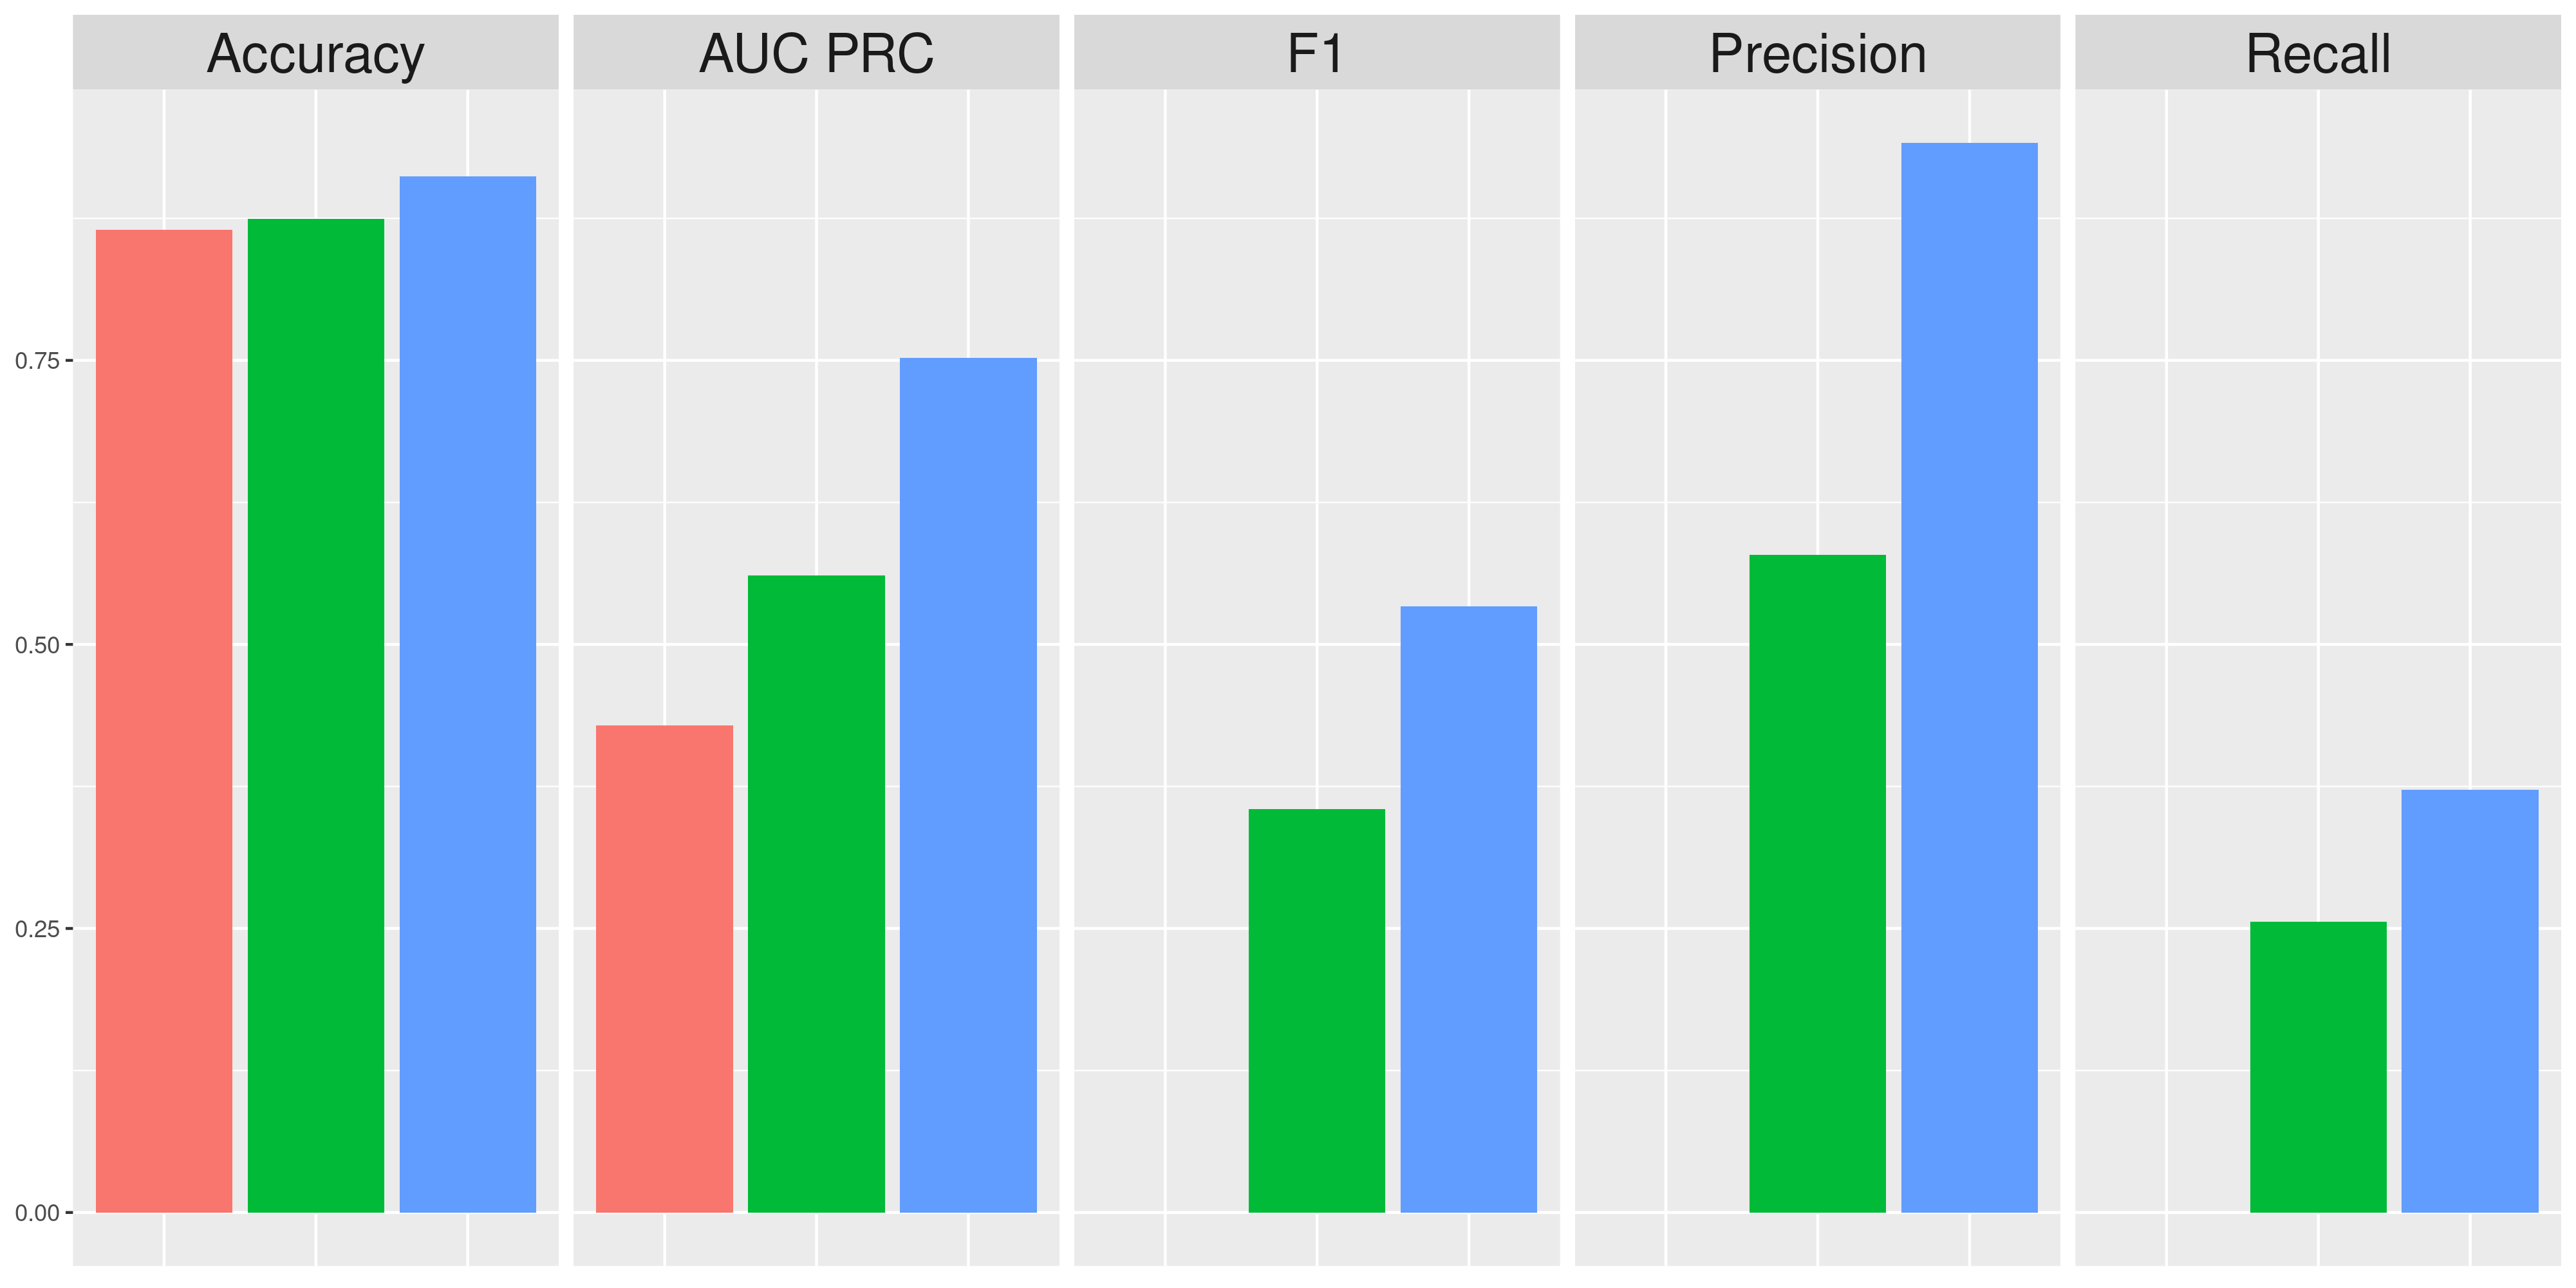
\includegraphics[width=12cm, height=8cm, keepaspectratio]{images/comparison/outliers/kernel/z-score_measures.png}
    }
    \quad
    \subfloat[Standardizzazione + PCA]{%
        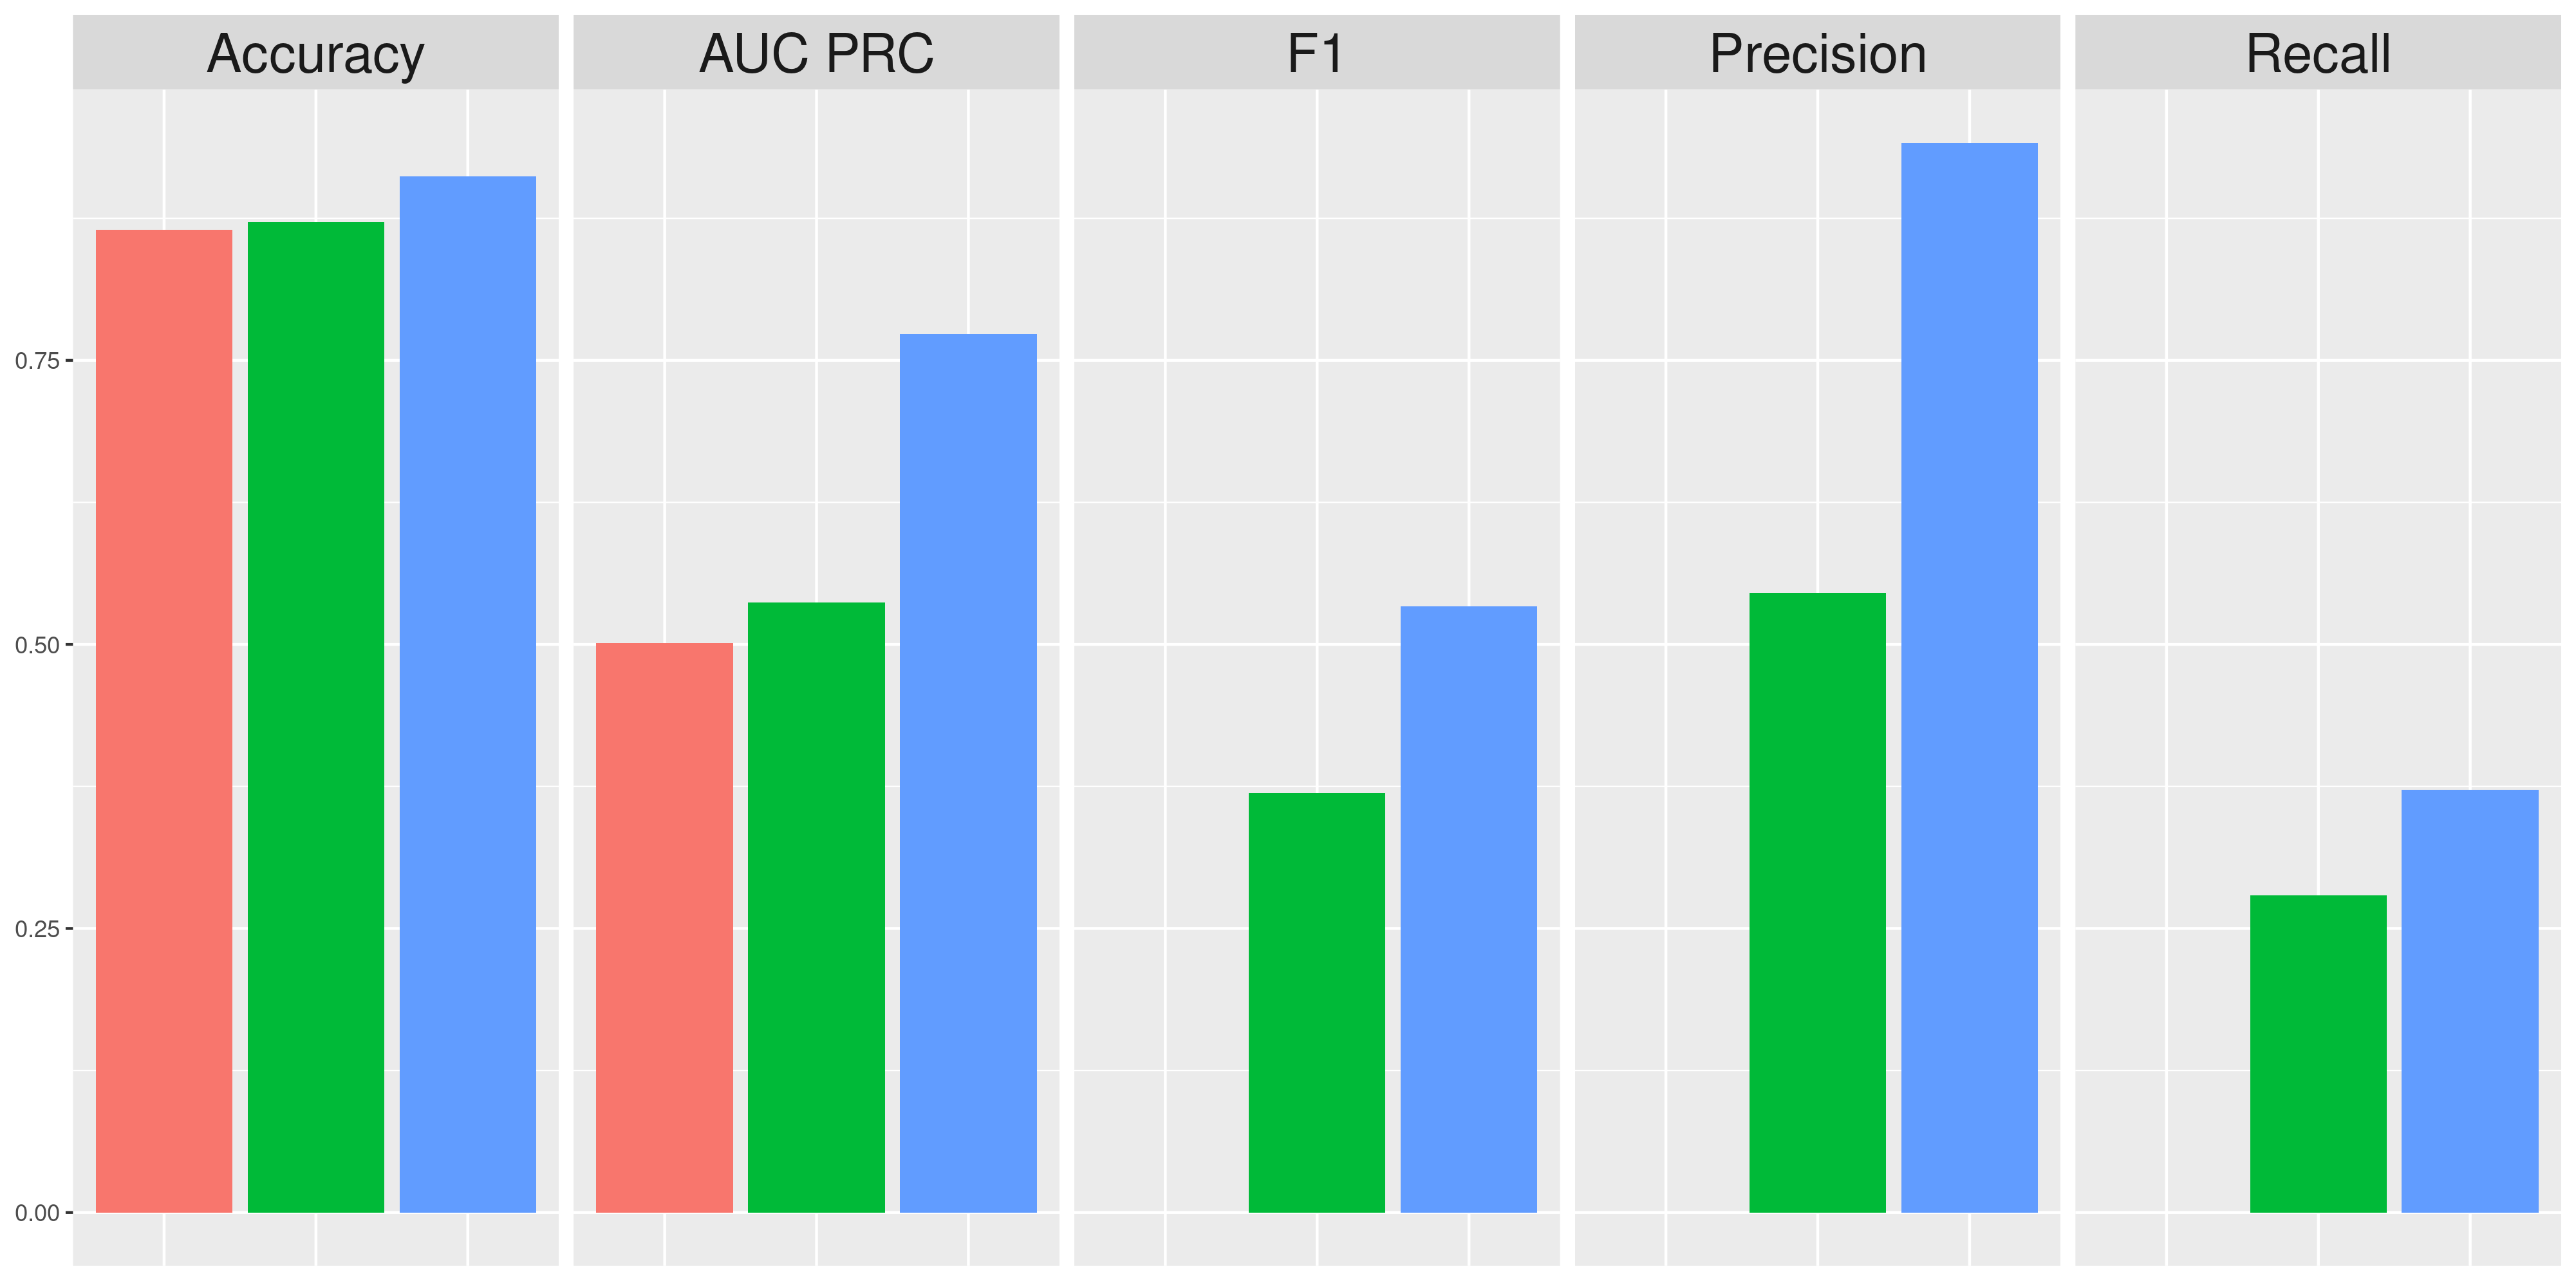
\includegraphics[width=12cm, height=8cm, keepaspectratio]{images/comparison/outliers/kernel/pca_measures.png}
    }

    \label{fig:measures_svm_outliers}
    \caption{Risultati della SVM con i diversi kernel (lineare: rosso, polinomiale: verde, radiale: blu) sul testset con outliers}
\end{figure}

\begin{figure}[H]
    \centering

    \subfloat[Standardizzazione]{%
        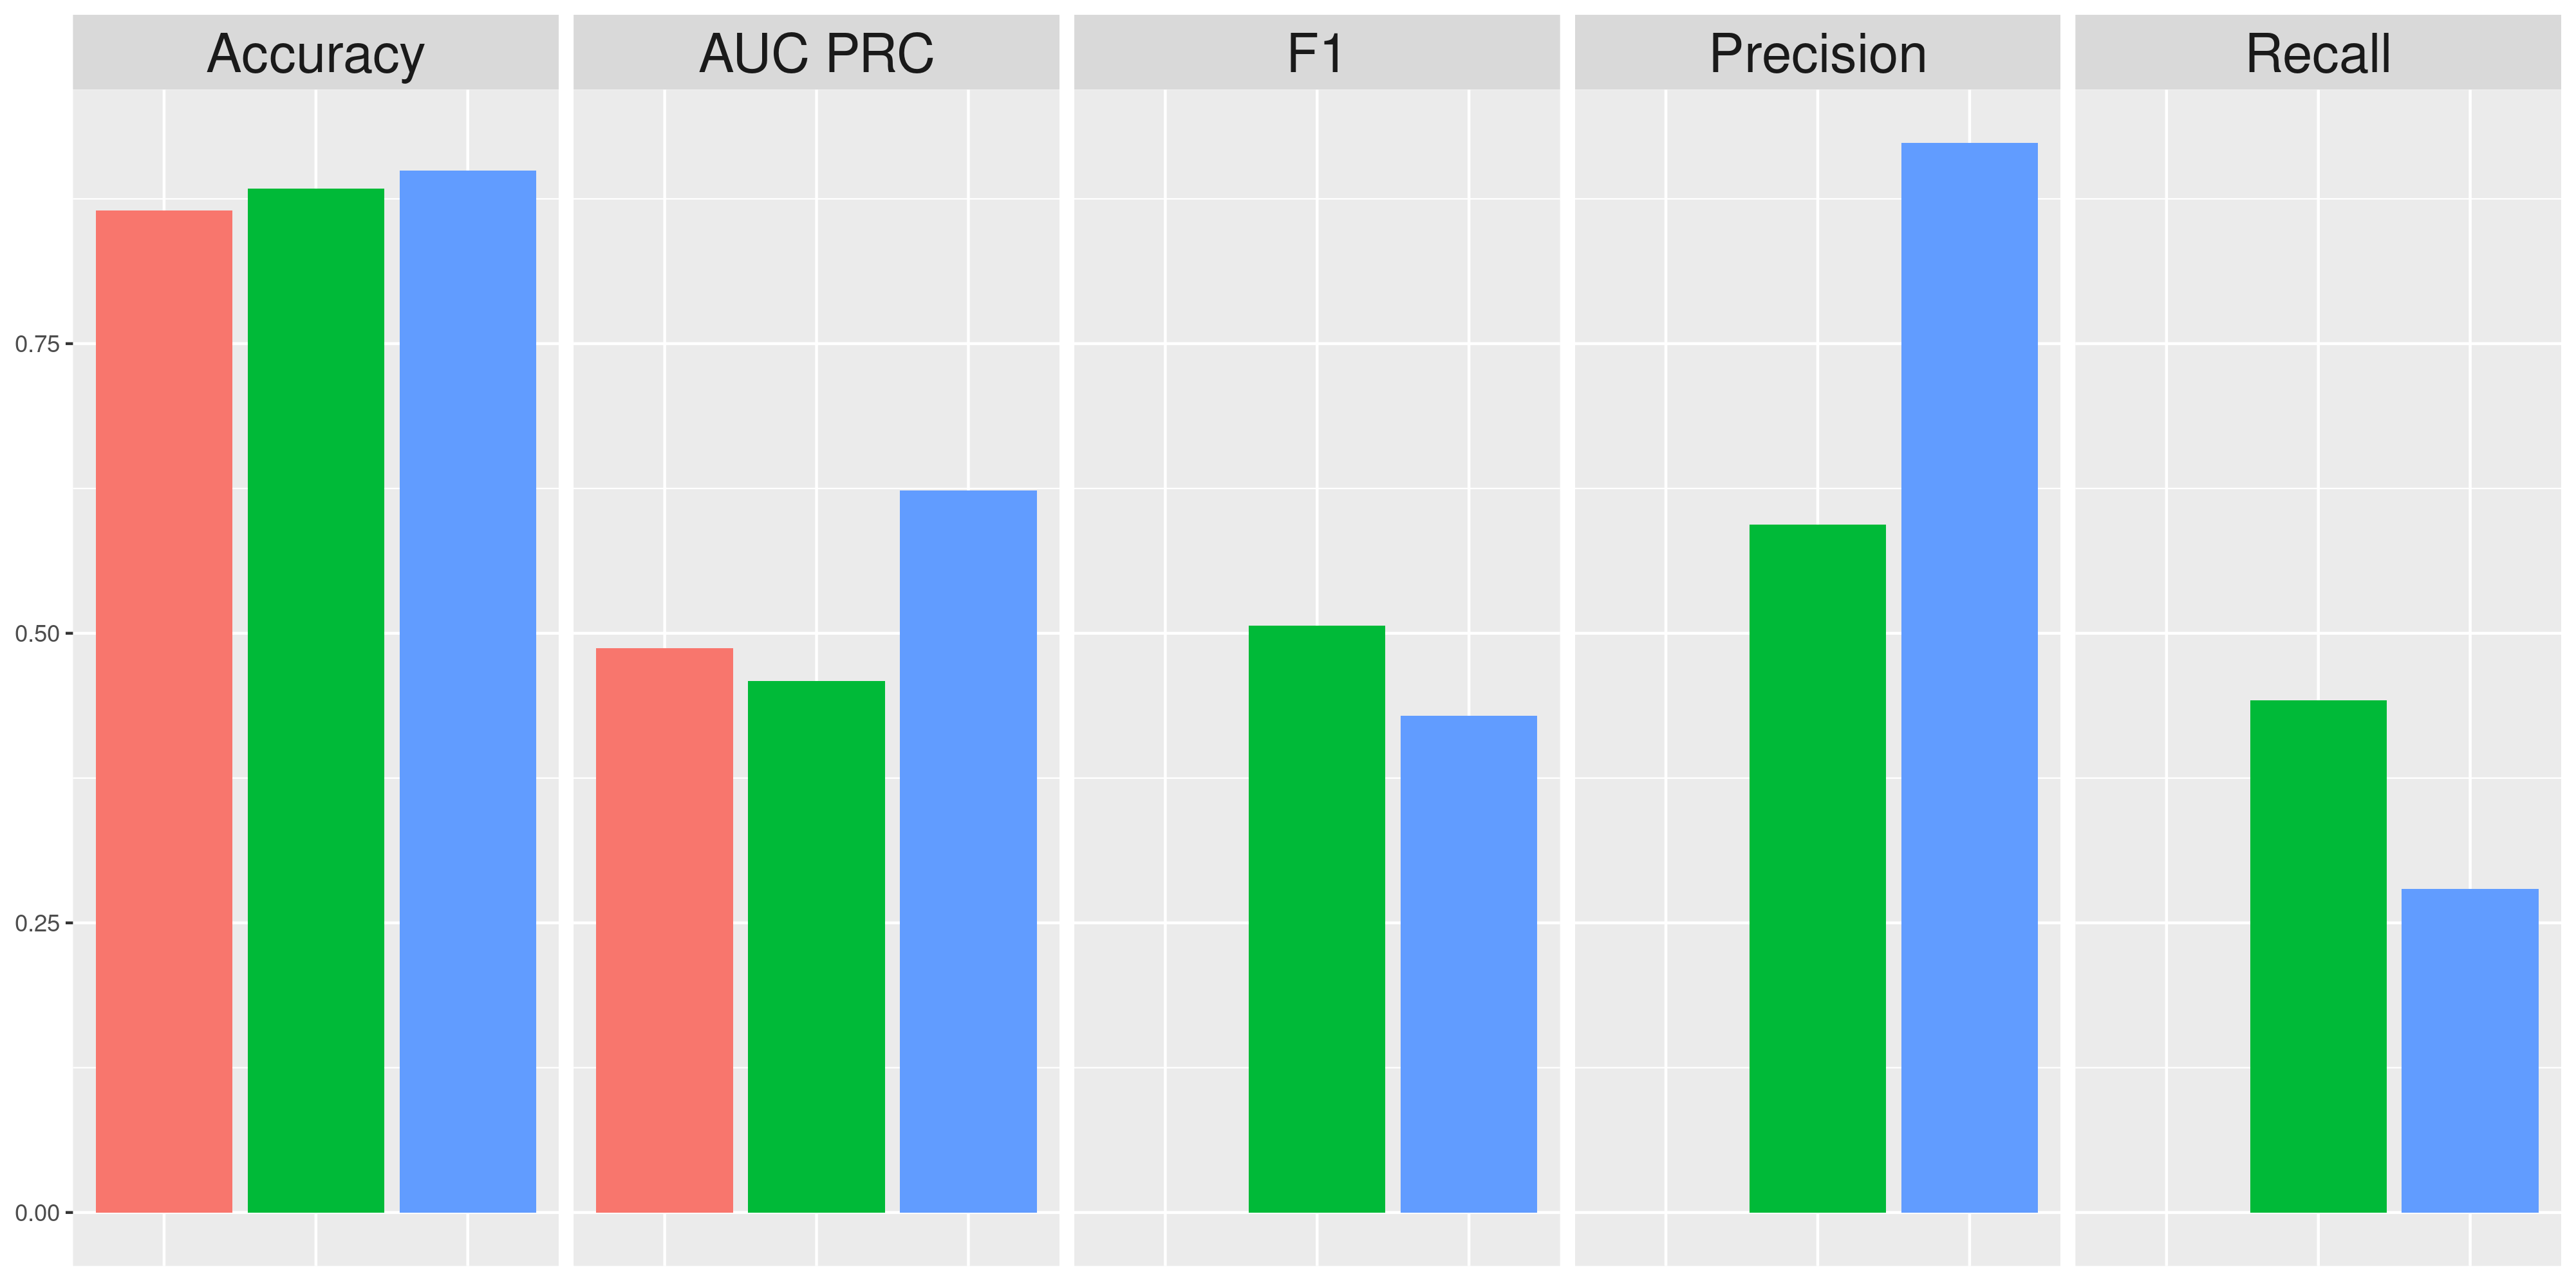
\includegraphics[width=12cm, height=8cm, keepaspectratio]{images/comparison/no-outliers/kernel/z-score_measures.png}
    }
    \quad
    \subfloat[Standardizzazione + PCA]{%
        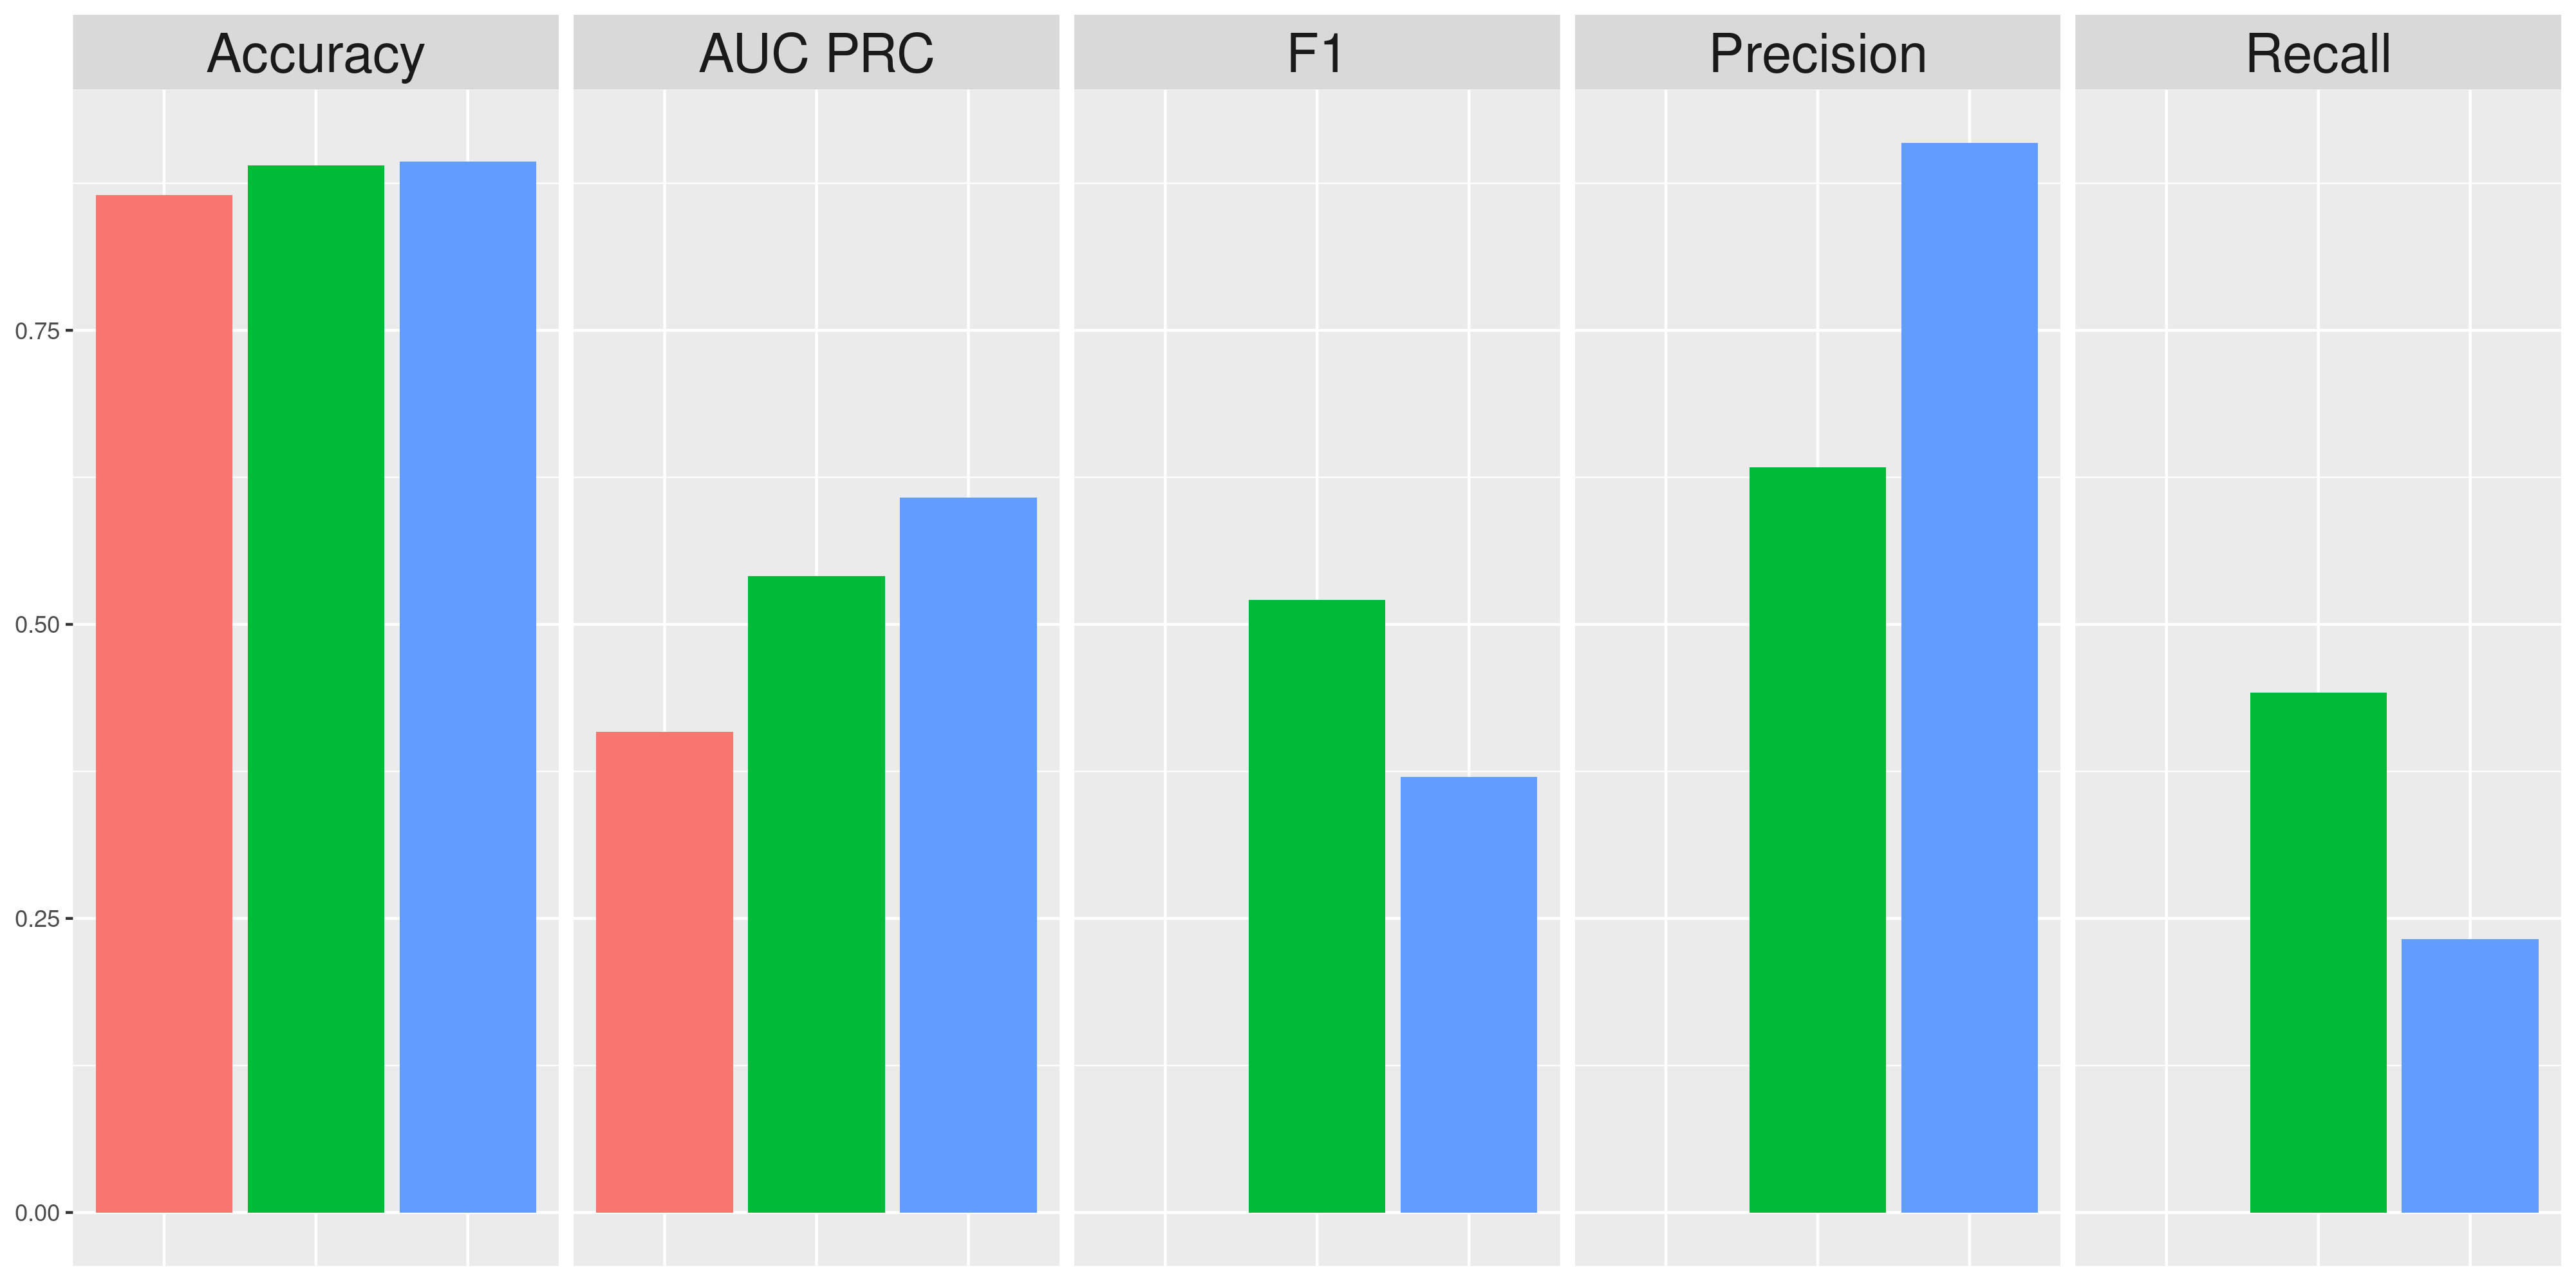
\includegraphics[width=12cm, height=8cm, keepaspectratio]{images/comparison/no-outliers/kernel/pca_measures.png}
    }

    \label{fig:measures_svm}
    \caption{Risultati della SVM con i diversi kernel (lineare: rosso, polinomiale: verde, radiale: blu) sul testset senza outliers}
\end{figure}

\noindent
Mostriamo ora graficamente la curva ROC (Receiver Operating Characteristic) e la PRC (Precision Recall Curve) che è più sensibile a situazioni con dati sbilanciati.
Infatti si può notare come le differenze tra i vari modelli siano molto grandi rispetto alla PRC, invece rispetto alla ROC tutti i modelli sono molto simili.
Inoltre la rimozione degli outliers comporta una perdita drastica nelle performance dei modelli.

\newpage

\begin{figure}[H]
    \centering

    \subfloat[Standardizzazione]{%
        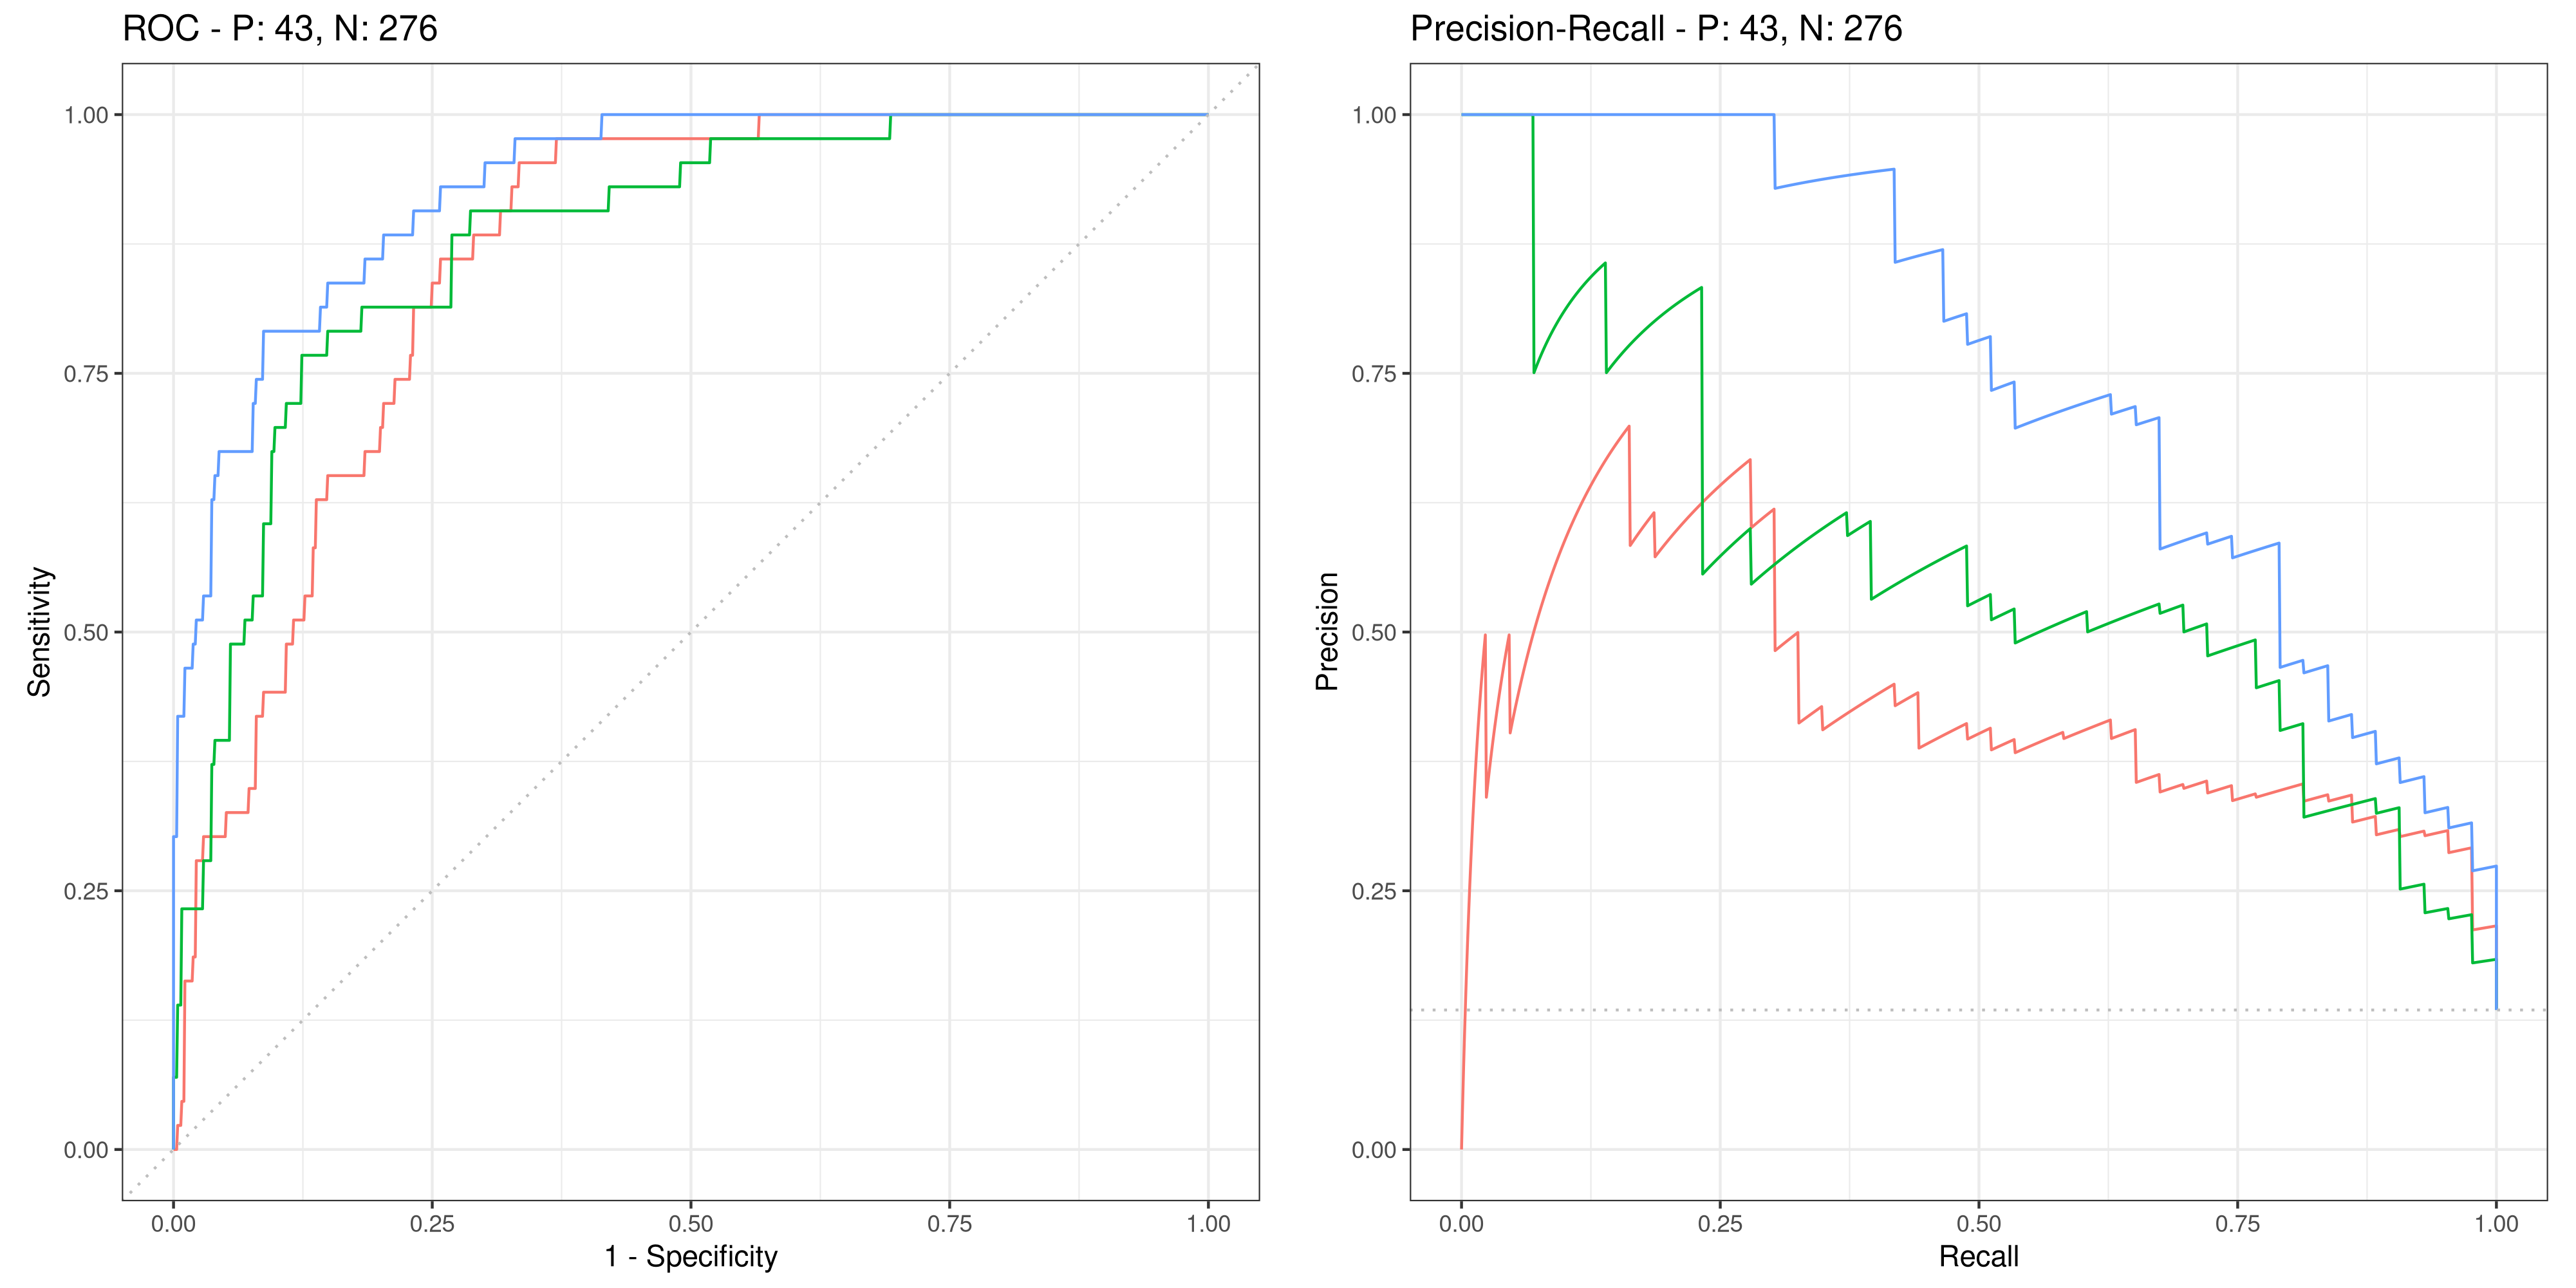
\includegraphics[width=\linewidth]{images/roc/outliers/kernel/z-score.png}
    }
    \quad
    \subfloat[Standardizzazione + PCA]{%
        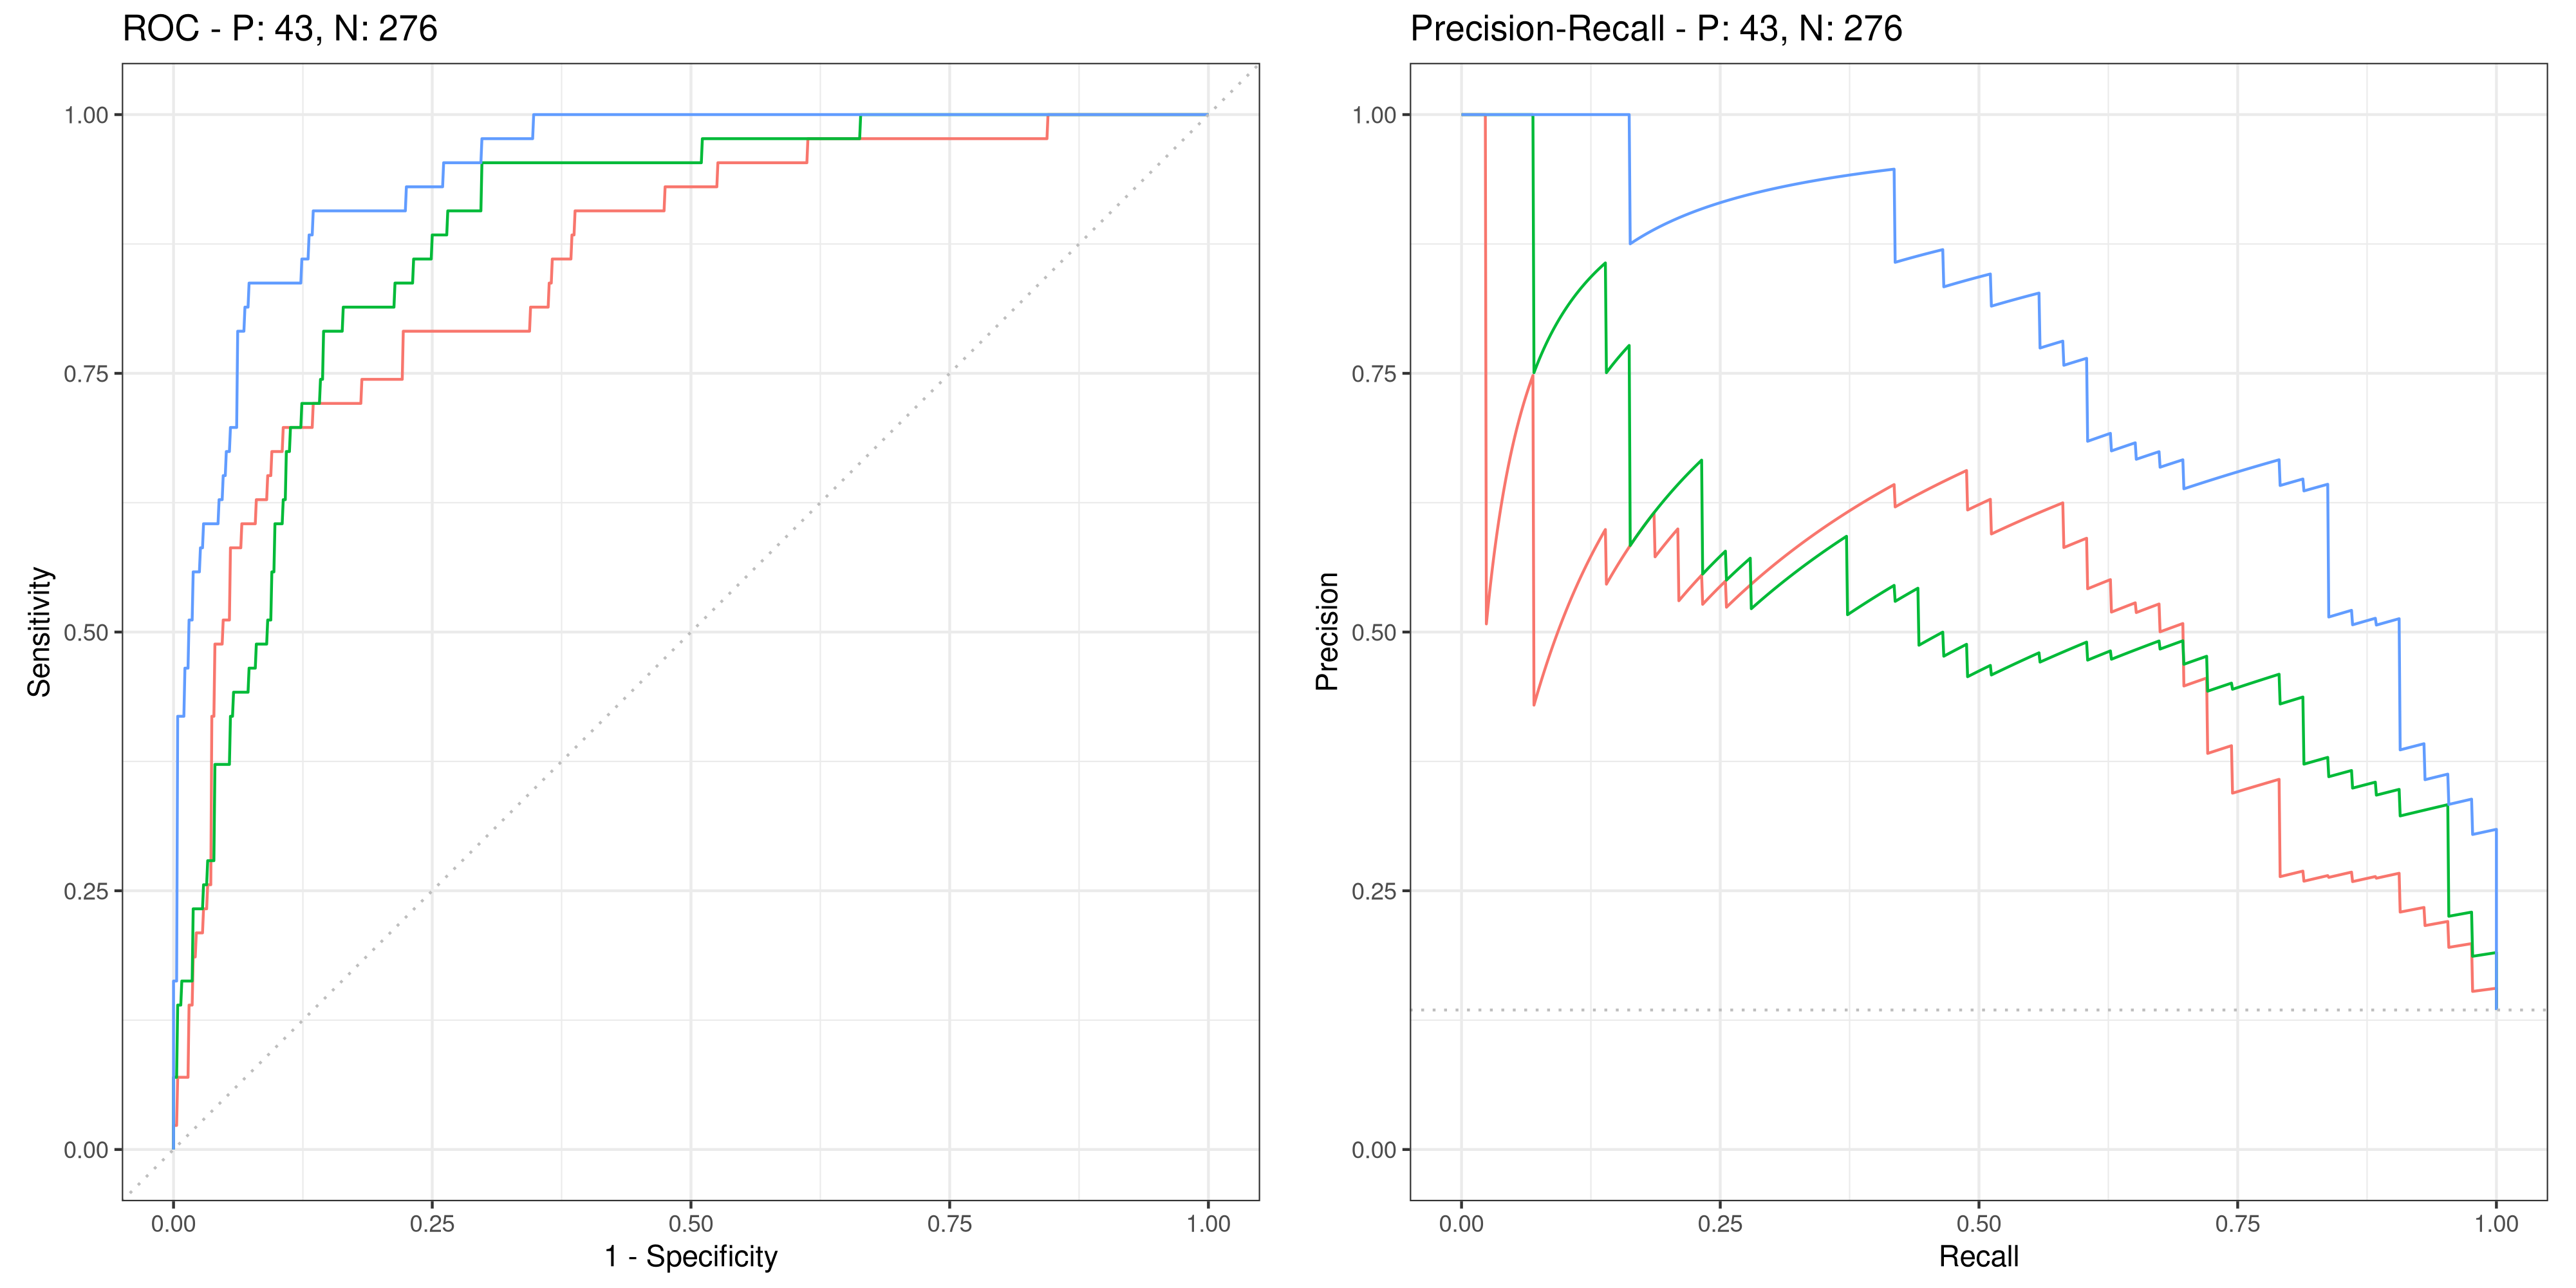
\includegraphics[width=\linewidth]{images/roc/outliers/kernel/pca.png}
    }
    \label{fig:roc_svm_outliers}
    \caption{Curve ROC e PRC per i diversi kernel (lineare: rosso, polinomiale: verde, radiale: blu) sul testset con outliers}
\end{figure}

\begin{figure}[H]
    \centering

    \subfloat[Standardizzazione]{%
        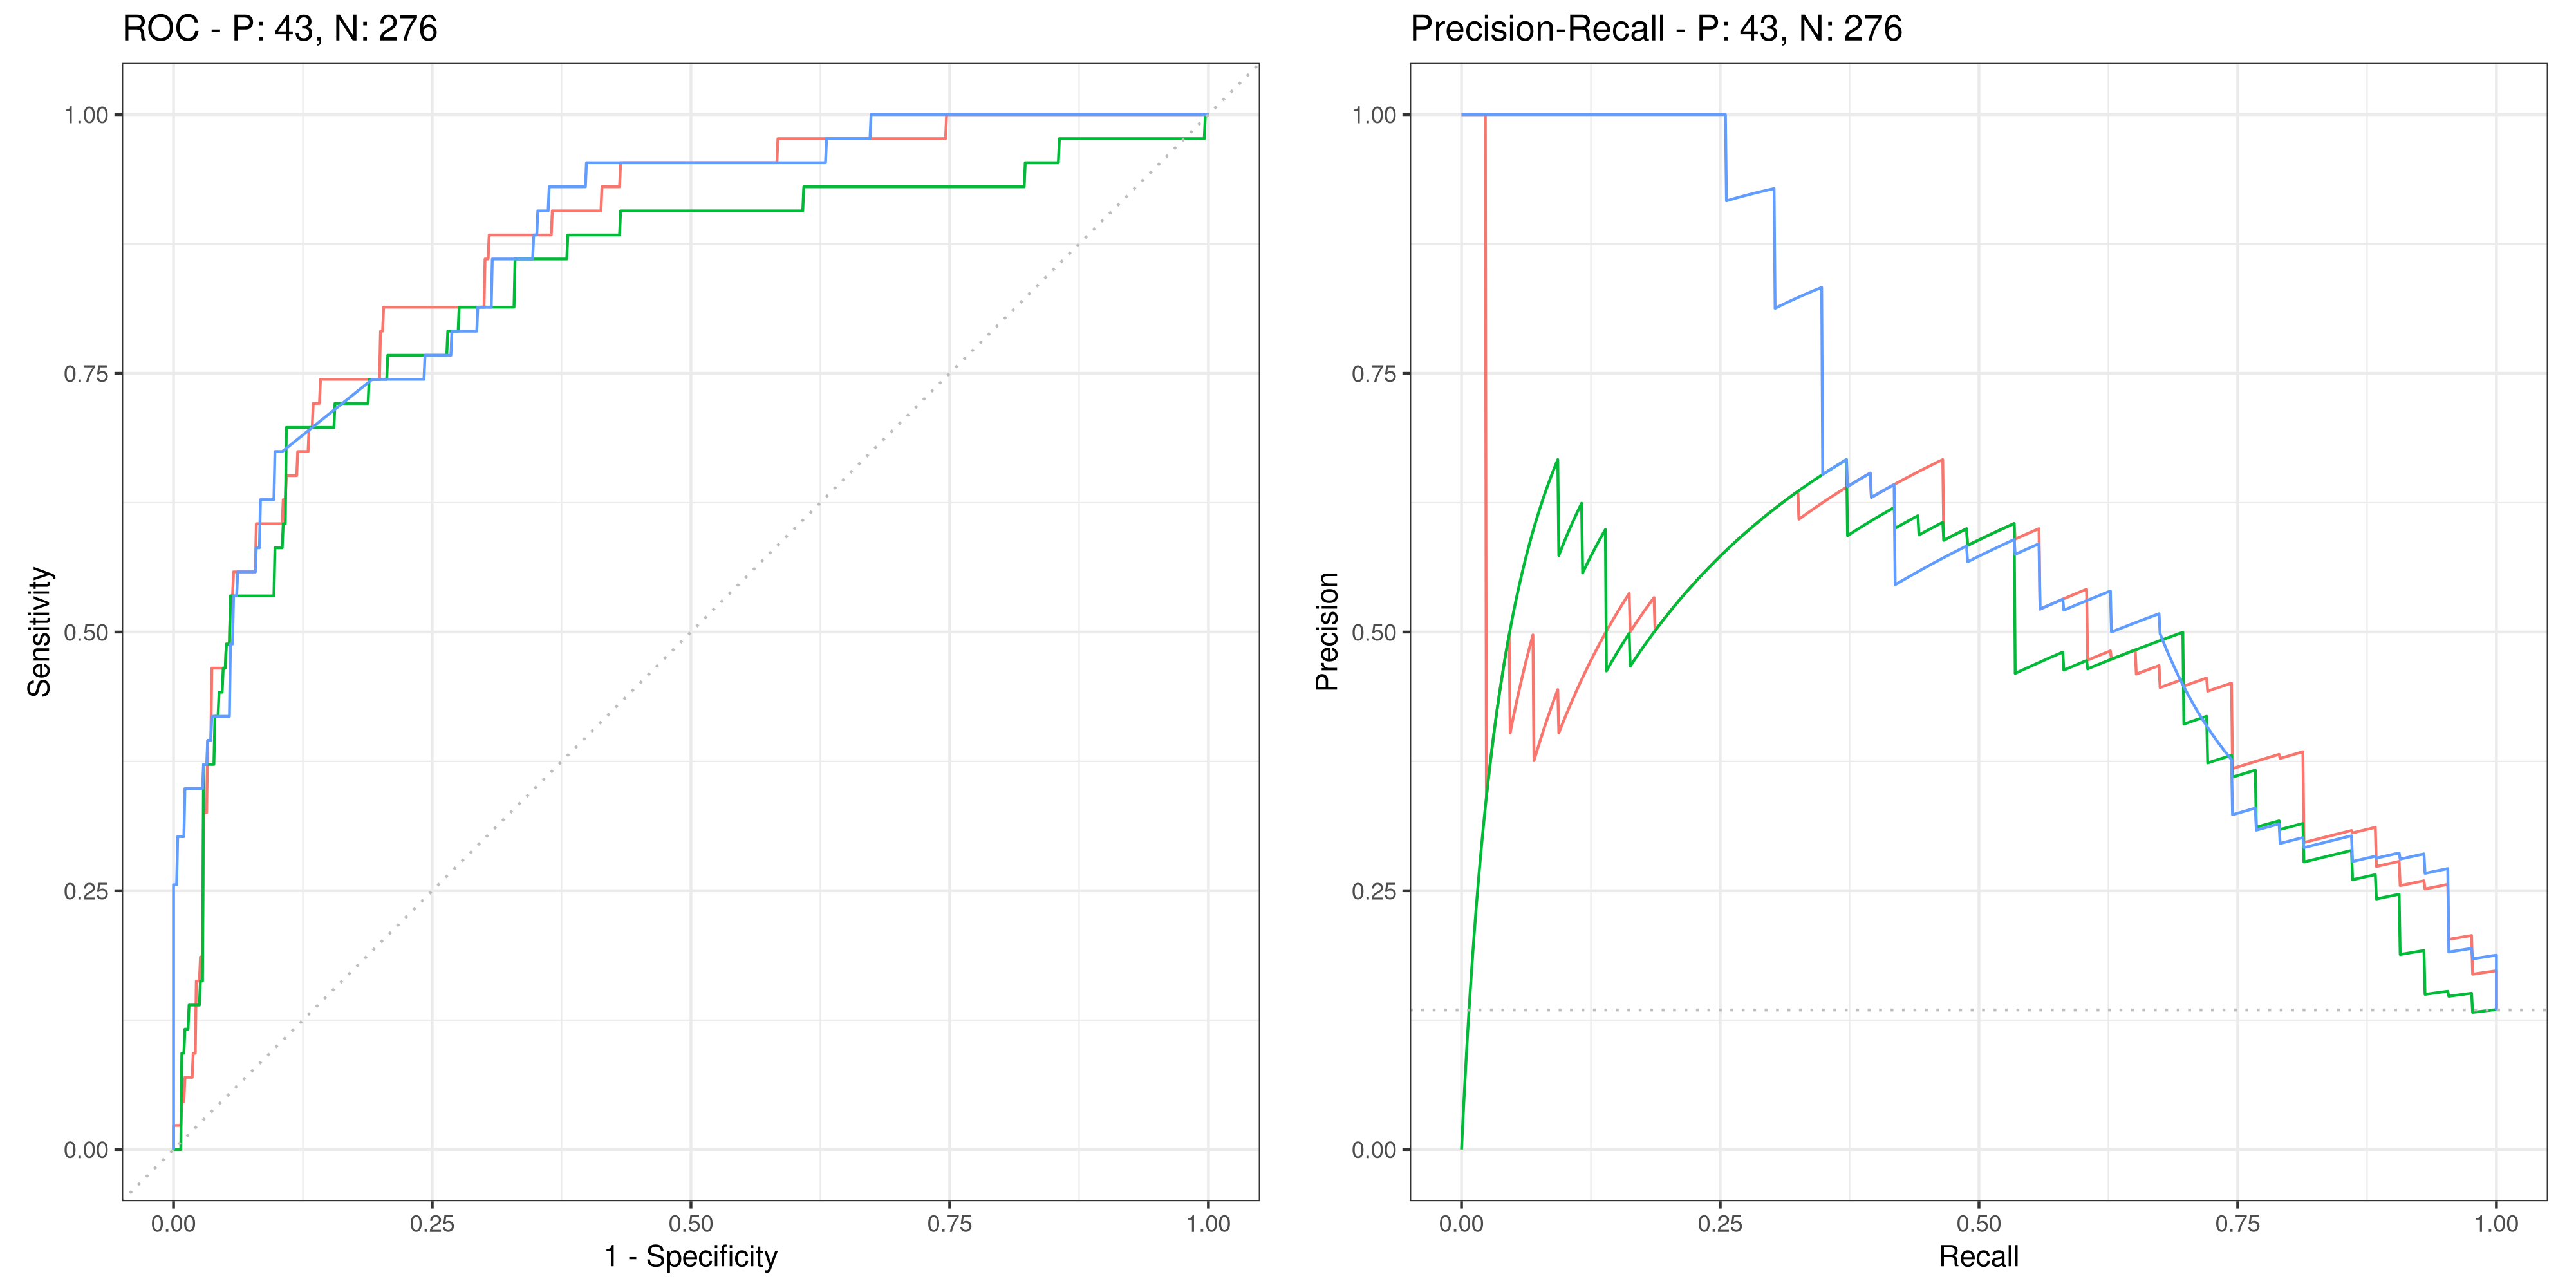
\includegraphics[width=\linewidth]{images/roc/no-outliers/kernel/z-score.png}
    }
    \quad
    \subfloat[Standardizzazione + PCA]{%
        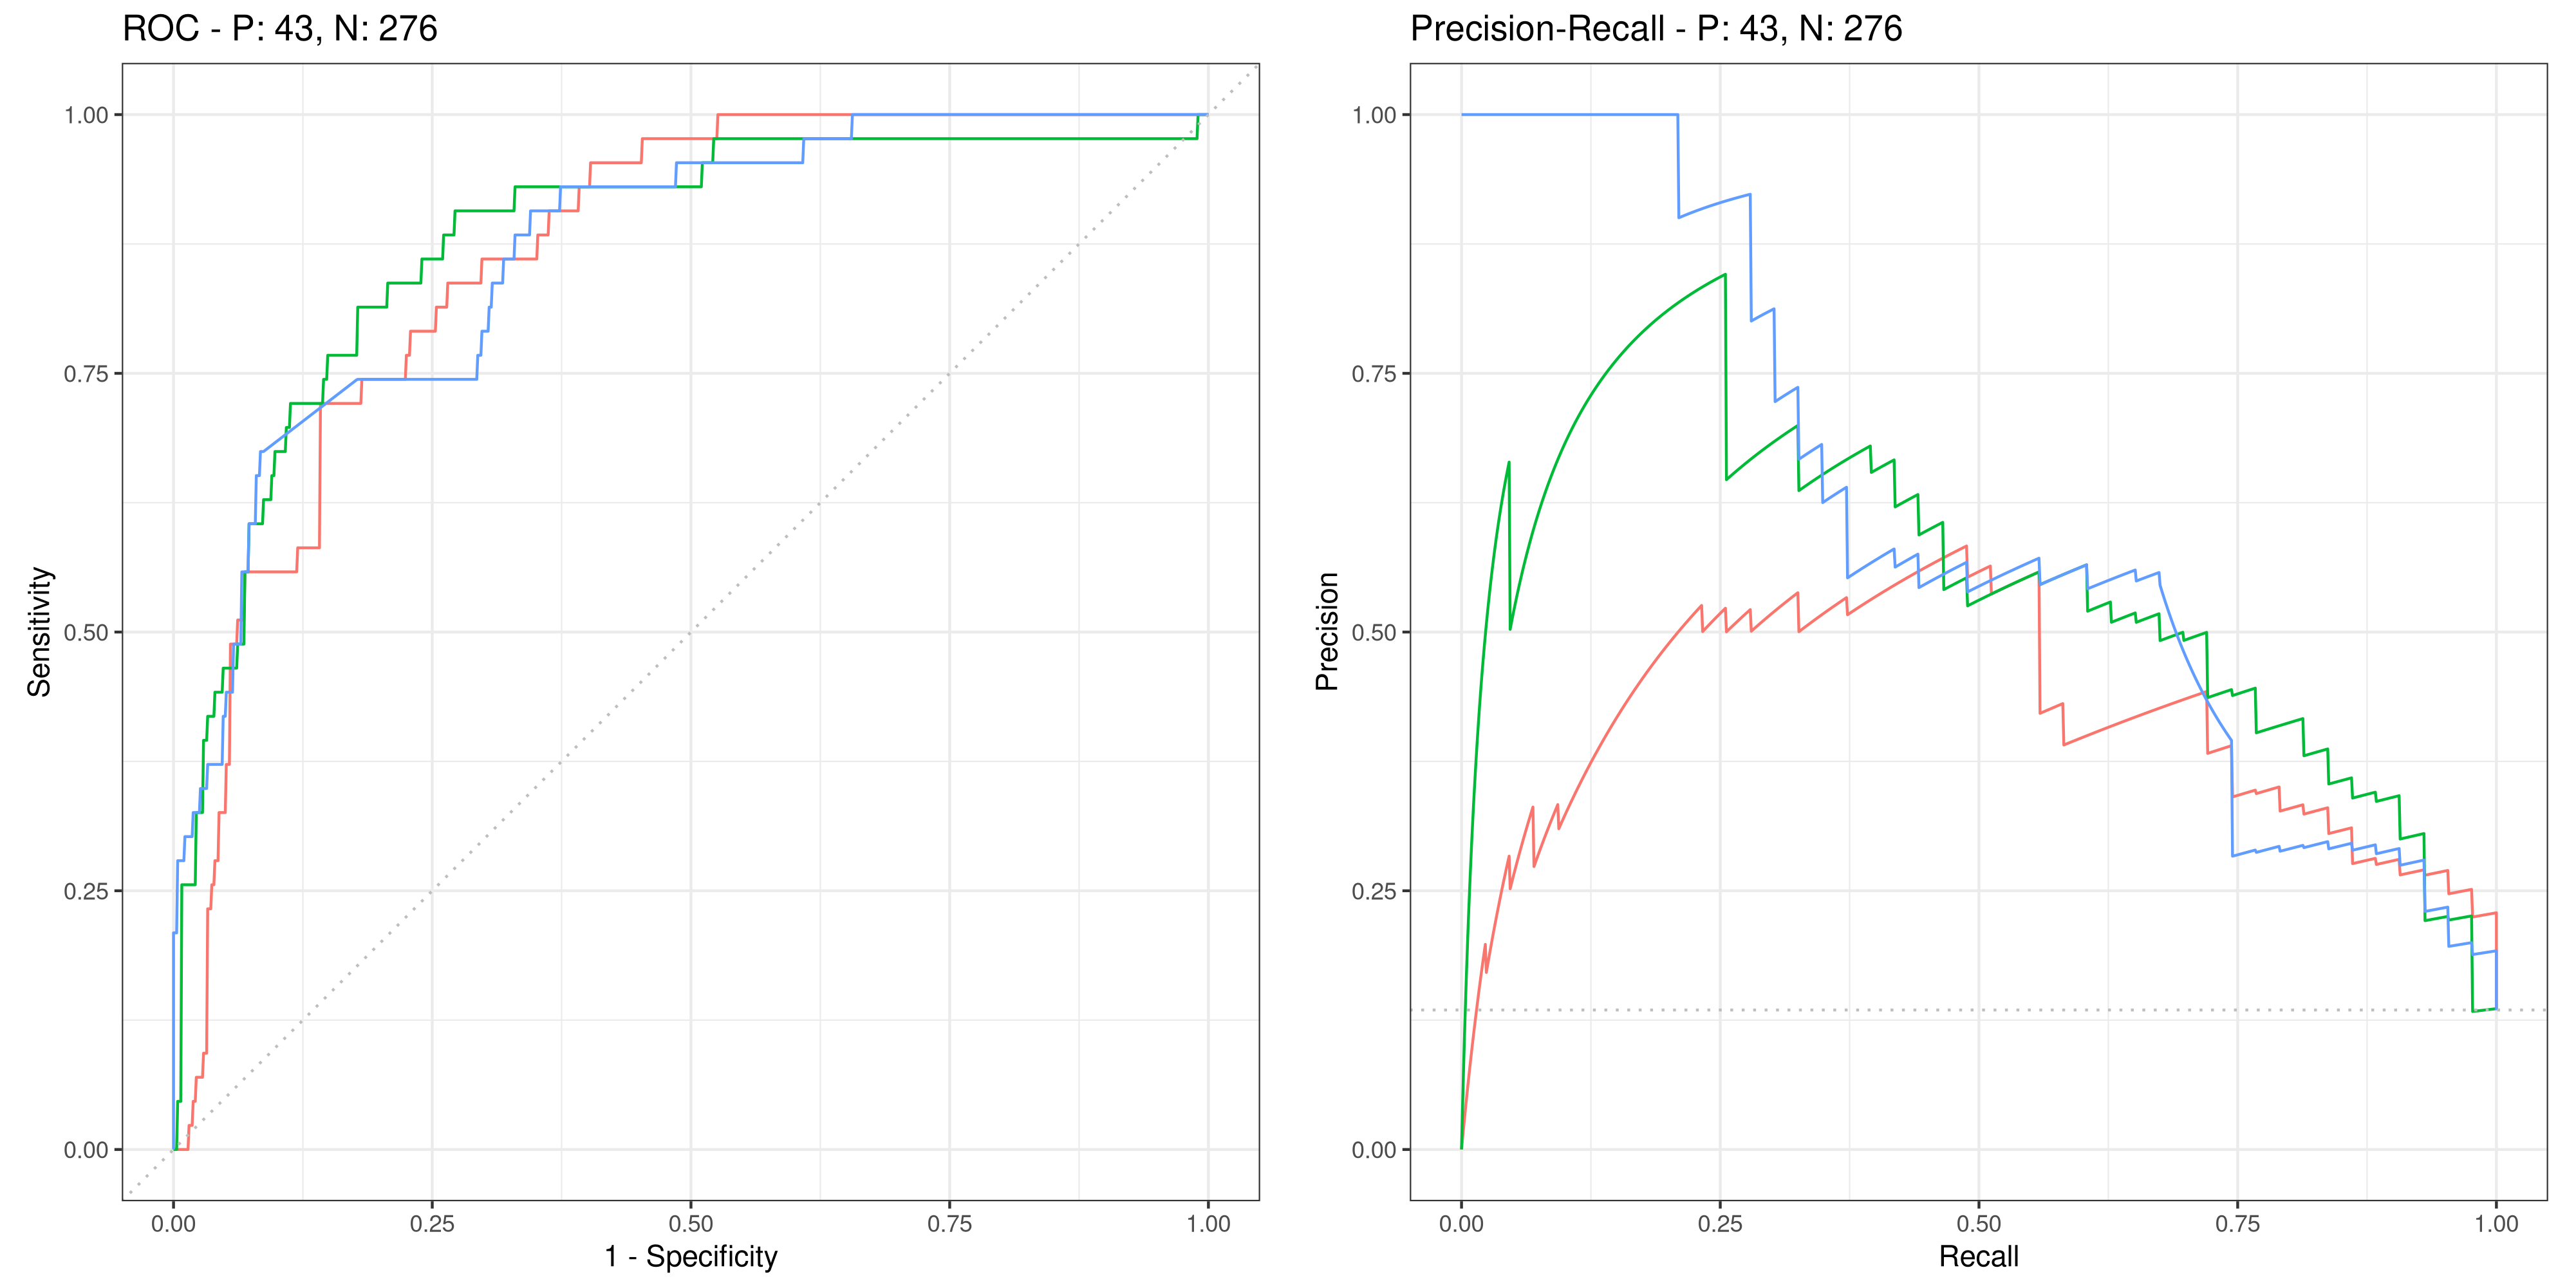
\includegraphics[width=\linewidth]{images/roc/no-outliers/kernel/pca.png}
    }

    \label{fig:roc_svm}
    \caption{Curve ROC e PRC per i diversi kernel (lineare: rosso, polinomiale: verde, radiale: blu) sul testset senza outliers}
\end{figure}

\newpage

\noindent
Riassumendo nella seguente tabella è possibile vedere come il kernel radiale superi gli altri kernel mantenendo gli outliers, mentre effettuando la rimozione con il kernel polinomiale si assumono valori più alti di F1 e Recall.
E' possibile notare che la ROC e la PRC si abbassano drasticamente rimuovendo gli outliers.
Possiamo quindi concludere che l'SVM con kernel radiale, a prescindere dal pre processing, risulti il modello migliore nella maggioranza dei casi analizzati.

\begin{table}[H]
\centering
\resizebox{\textwidth}{!}{%
\begin{tabular}{@{}ccccccccc@{}}
\toprule
\textbf{Kernel} & \textbf{Overall Accuracy} & \textbf{Precision} & \textbf{Recall} & \textbf{F1} & \textbf{ROC AUC} & \textbf{PRC AUC} & \textbf{95\% CI} & \textbf{P-Value} \\ \midrule
lineare & 0.8652 & NA & 0 & NA & 0.8604651 & 0.4288328 & (0.8228, 0.9007) & 0.5405 \\
polinomiale & 0.8746 & 0.57895 & 0.25581 & 0.35484 & 0.8795079 & 0.5608824 & (0.8332, 0.9089) & 0.3471558 \\
radiale & \textbf{0.9122} & \textbf{0.94118} & \textbf{0.37209} & \textbf{0.53333} & \textbf{0.9313279} & \textbf{0.7520759} & (0.8756, 0.9409) & 0.006404 \\ \bottomrule
\end{tabular}%
}
\caption{Risultati dei diversi kernel sul testset con Standardizzazione}
\label{tab:my-table}
\end{table}

\begin{table}[H]
\centering
\resizebox{\textwidth}{!}{%
\begin{tabular}{@{}ccccccccc@{}}
\toprule
\textbf{Kernel} & \textbf{Overall Accuracy} & \textbf{Precision} & \textbf{Recall} & \textbf{F1} & \textbf{ROC AUC} & \textbf{PRC AUC} & \textbf{95\% CI} & \textbf{P-Value} \\ \midrule
lineare & 0.8652 & NA & 0 & NA & 0.8547354 & 0.5011905 & (0.8228, 0.9007) & 0.5405 \\
polinomiale & 0.8715 & 0.54545 & 0.27907 & 0.36923 & 0.8844793 & 0.5368917 & (0.8297, 0.9062) & 0.410227 \\
radiale & \textbf{0.9122} & \textbf{0.94118} & \textbf{0.37209} & \textbf{0.53333} & \textbf{0.9469161} & \textbf{0.7732596} & (0.8756, 0.9409) & 0.006404 \\ \bottomrule
\end{tabular}%
}
\caption{Risultati dei diversi kernel sul testset con Standardizzazione + PCA}
\label{tab:my-table}
\end{table}

\begin{table}[H]
\centering
\resizebox{\textwidth}{!}{%
\begin{tabular}{@{}ccccccccc@{}}
\toprule
\textbf{Kernel} & \textbf{Overall Accuracy} & \textbf{Precision} & \textbf{Recall} & \textbf{F1} & \textbf{ROC AUC} & \textbf{PRC AUC} & \textbf{95\% CI} & \textbf{P-Value} \\ \midrule
lineare & 0.8652 & NA & 0 & NA & 0.8681328 & 0.4870888 & (0.8228, 0.9007) & 0.5405 \\
polinomiale & 0.884 & 0.59375 & \textbf{0.44186} & \textbf{0.50667} & 0.8313953 & 0.4587525 & (0.8437, 0.917) & 0.1845 \\
radiale & \textbf{0.8997} & \textbf{0.92308} & 0.27907 & 0.42857 & \textbf{0.8711662} & \textbf{0.6230968} & (0.8613, 0.9304) & 0.03864 \\ \bottomrule
\end{tabular}%
}
\caption{Risultati dei diversi kernel sul testset con Standardizzazione e rimozione outliers}
\label{tab:my-table}
\end{table}

\begin{table}[H]
\centering
\resizebox{\textwidth}{!}{%
\begin{tabular}{@{}ccccccccc@{}}
\toprule
\textbf{Kernel} & \textbf{Overall Accuracy} & \textbf{Precision} & \textbf{Recall} & \textbf{F1} & \textbf{ROC AUC} & \textbf{PRC AUC} & \textbf{95\% CI} & \textbf{P-Value} \\ \midrule
lineare & 0.8652 & NA & 0 & NA & 0.8624031 & 0.408548 & (0.8228, 0.9007) & 0.5405 \\
polinomiale & 0.8903 & 0.63333 & \textbf{0.44186} & \textbf{0.52055} & \textbf{0.878244} & 0.5411327 & (0.8507, 0.9224) & 0.10722 \\
radiale & \textbf{0.8934} & \textbf{0.90909} & 0.23256 & 0.37037 & 0.8684277 & \textbf{0.6079154} & (0.8543, 0.9251) & 0.07852 \\ \bottomrule
\end{tabular}%
}
\caption{Risultati dei diversi kernel sul testset con Standardizzazione + PCA e rimozione outliers}
\label{tab:my-table}
\end{table}


\newpage


\section{Confronto fra CART e SVM Radiale}
Così come già mostrato in precedenza per i kernel dell'SVM, vengono ora riportate le performance ottenute dall'SVM radiale e CART. Le metriche considerate sono Accuracy, AUC PRC, F1, Precision e Recall.
Da essi è possibile notare come, a parte il caso [\ref{fig:a}], l'SVM raggiunga i risultati migliori nella maggioranza dei casi.
Nel caso [\ref{fig:a}], invece è difficile dire quale dei due modelli sia il migliore dal momento che i risultati sono molto simili.


\begin{figure}[H]
    \centering

    \subfloat[Standardizzazione]{%
       \label{fig:a} 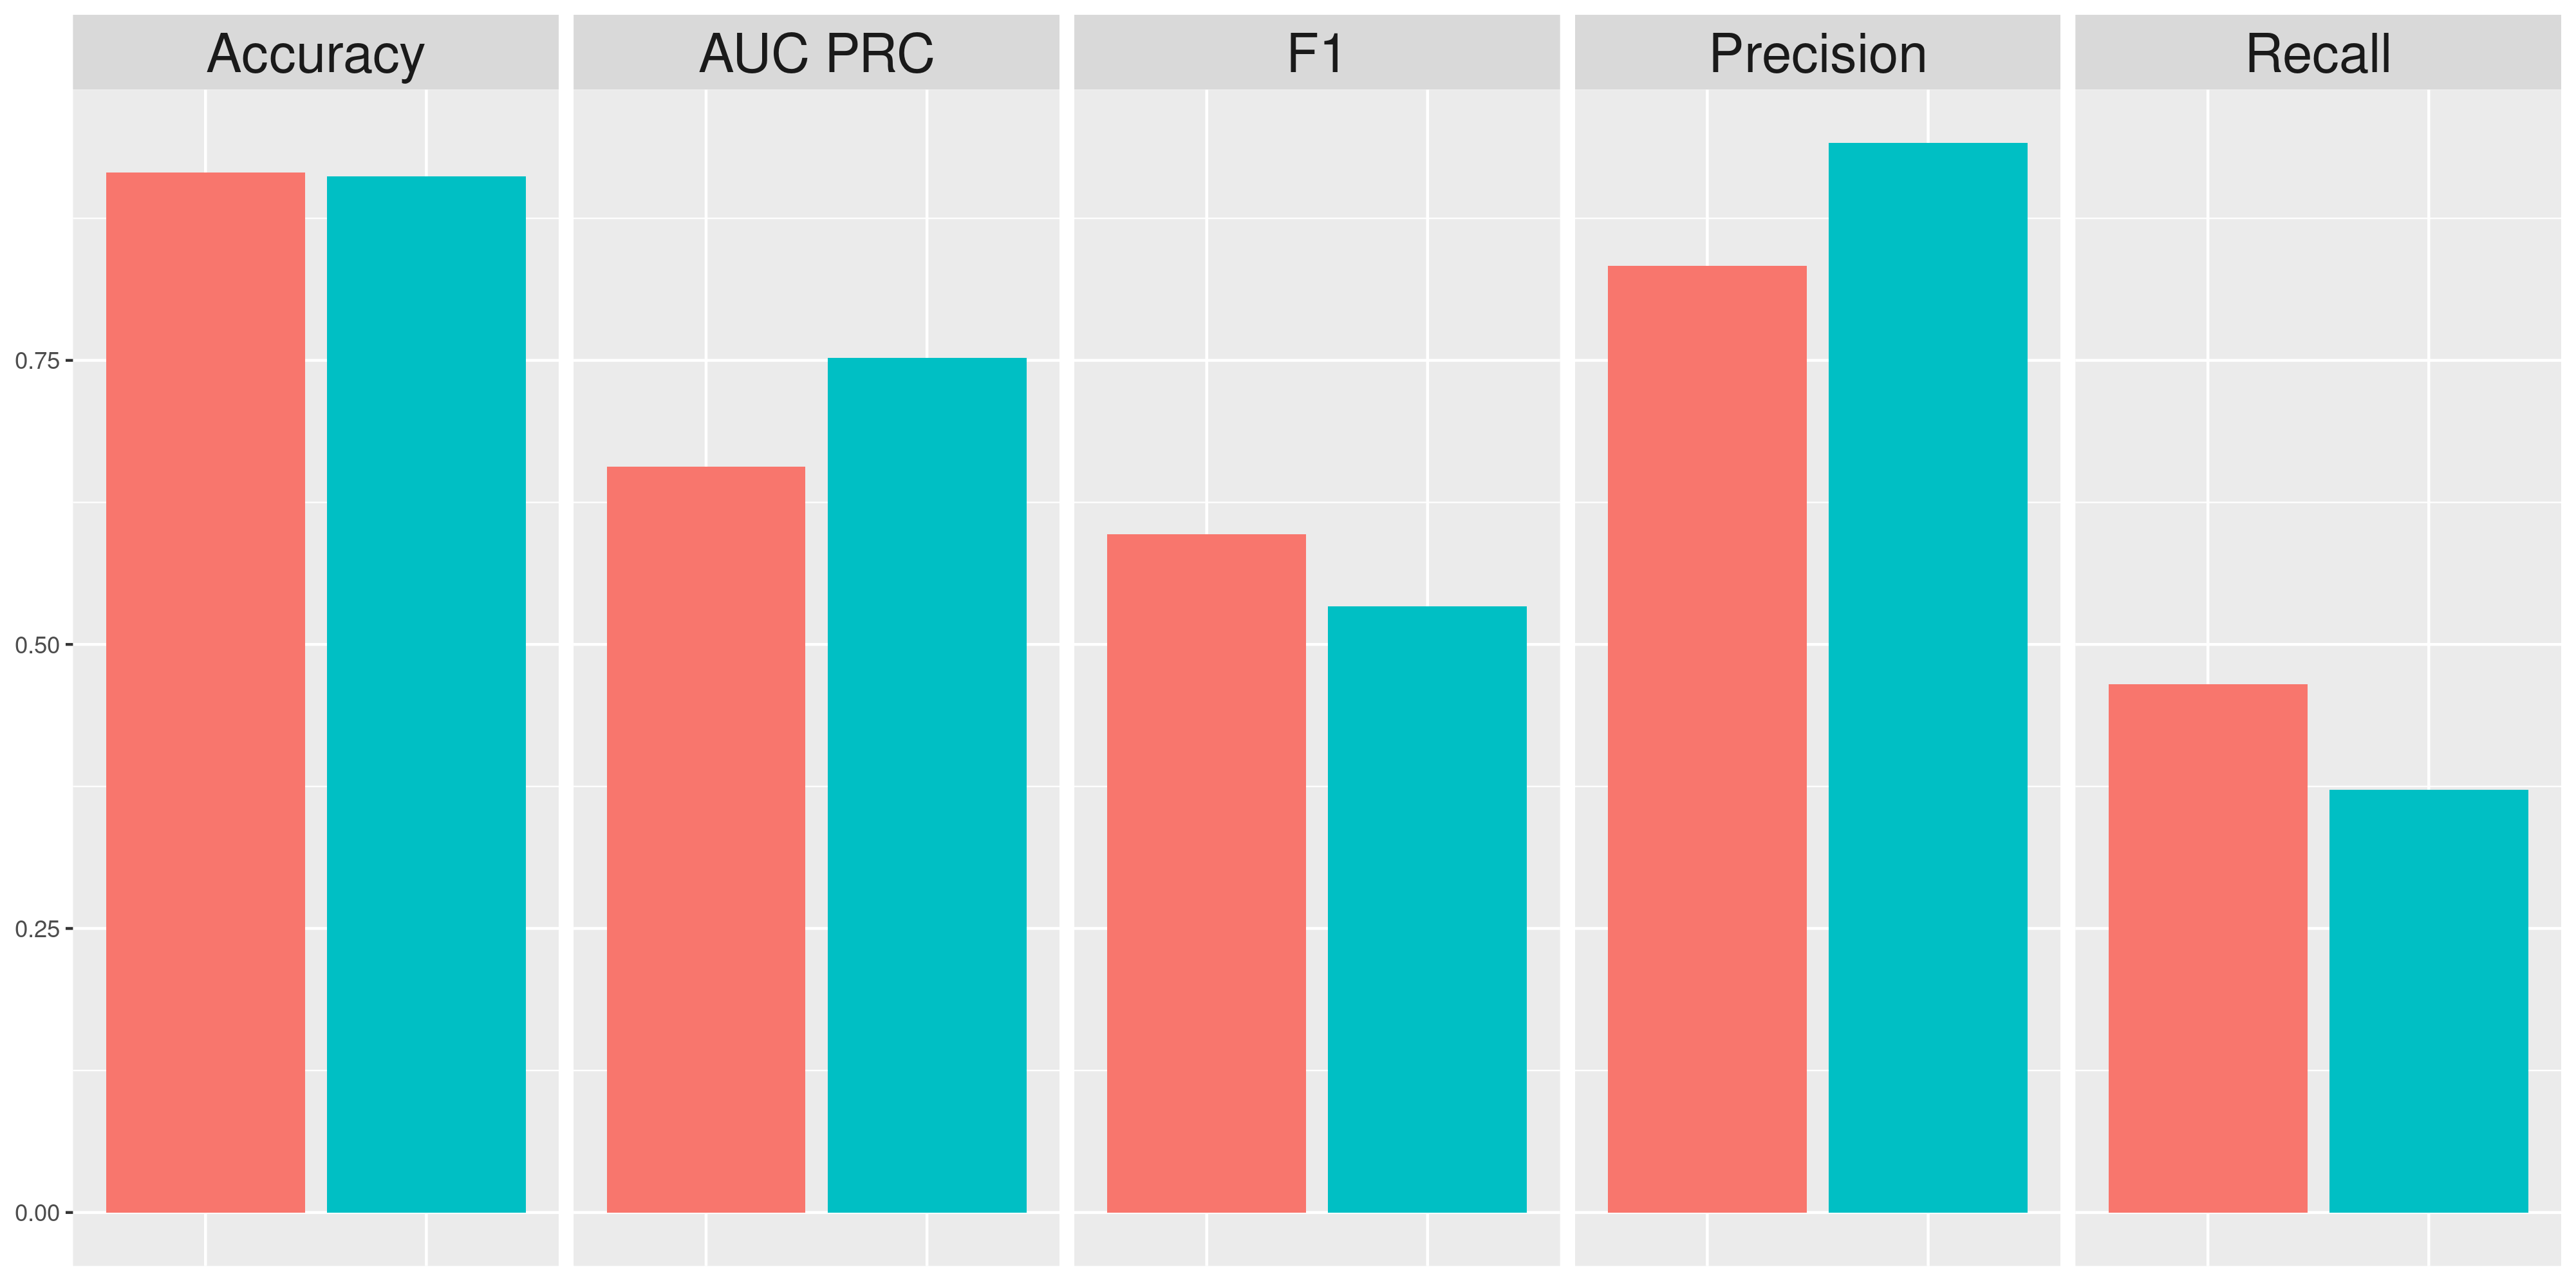
\includegraphics[width=12cm, height=8cm, keepaspectratio]{images/comparison/outliers/z-score_measures.png}
    }
    \quad
    \subfloat[Standardizzazione + PCA]{%
        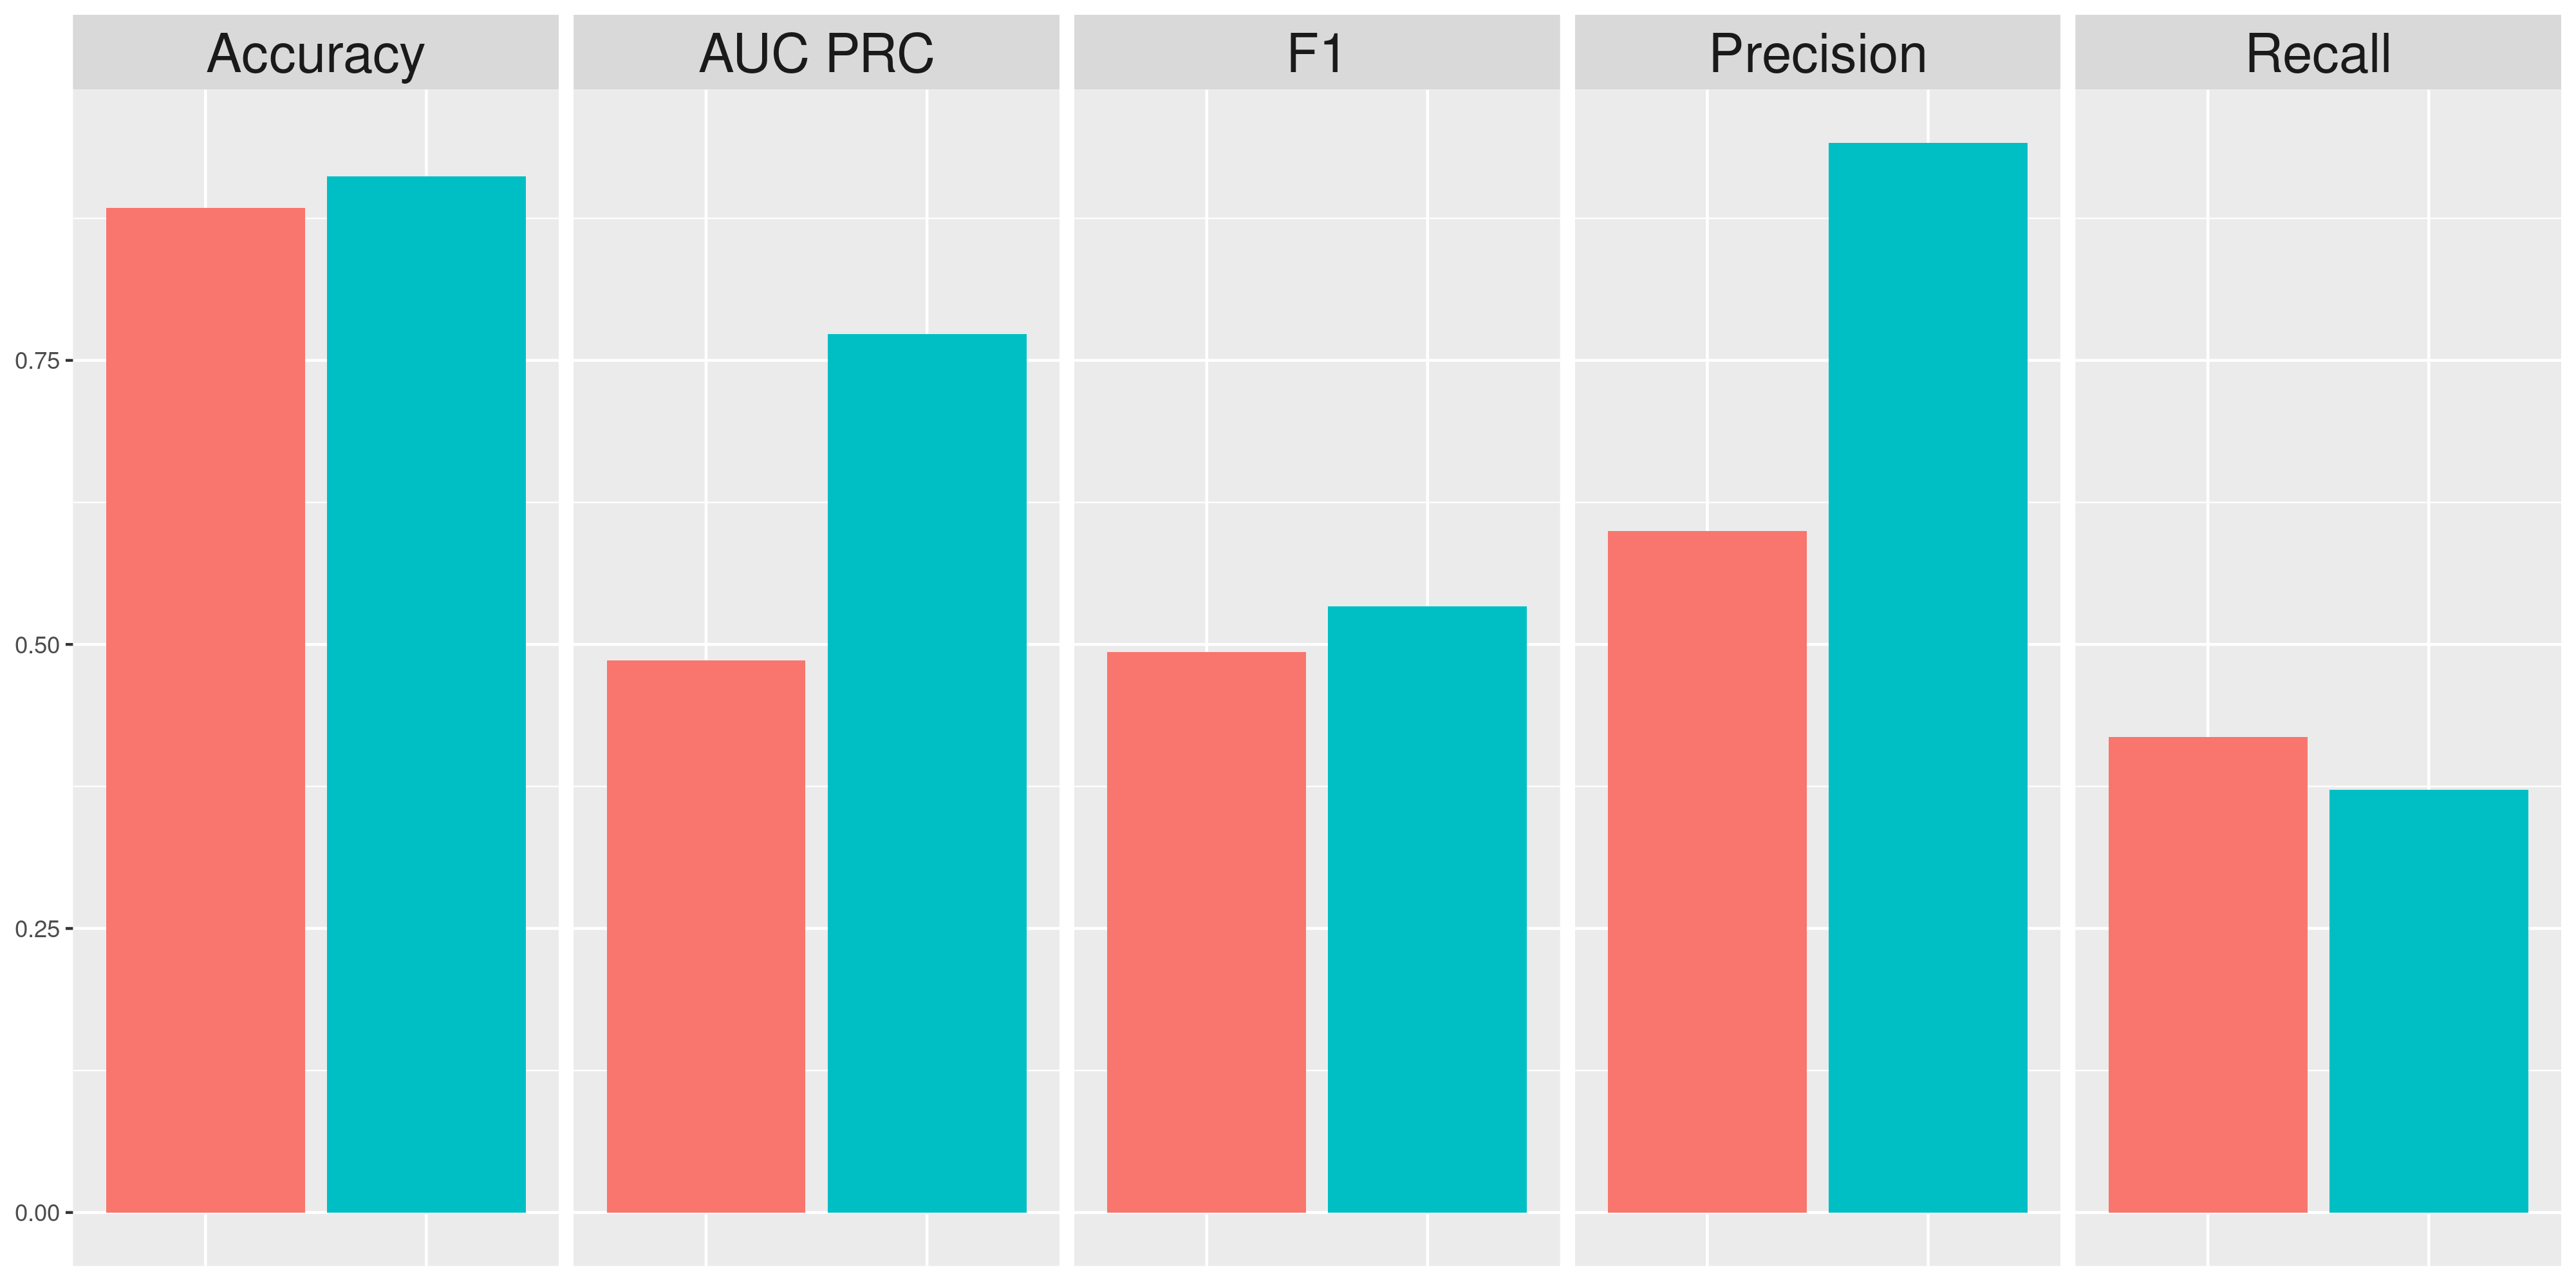
\includegraphics[width=12cm, height=8cm, keepaspectratio]{images/comparison/outliers/pca_measures.png}
    }

    \label{fig:measures_svm_outliers}
     \caption{Risultati dei due modelli (cart: rosso, radiale: blu) sul testset con outliers}
\end{figure}

\begin{figure}[H]
    \centering

    \subfloat[Standardizzazione]{%
        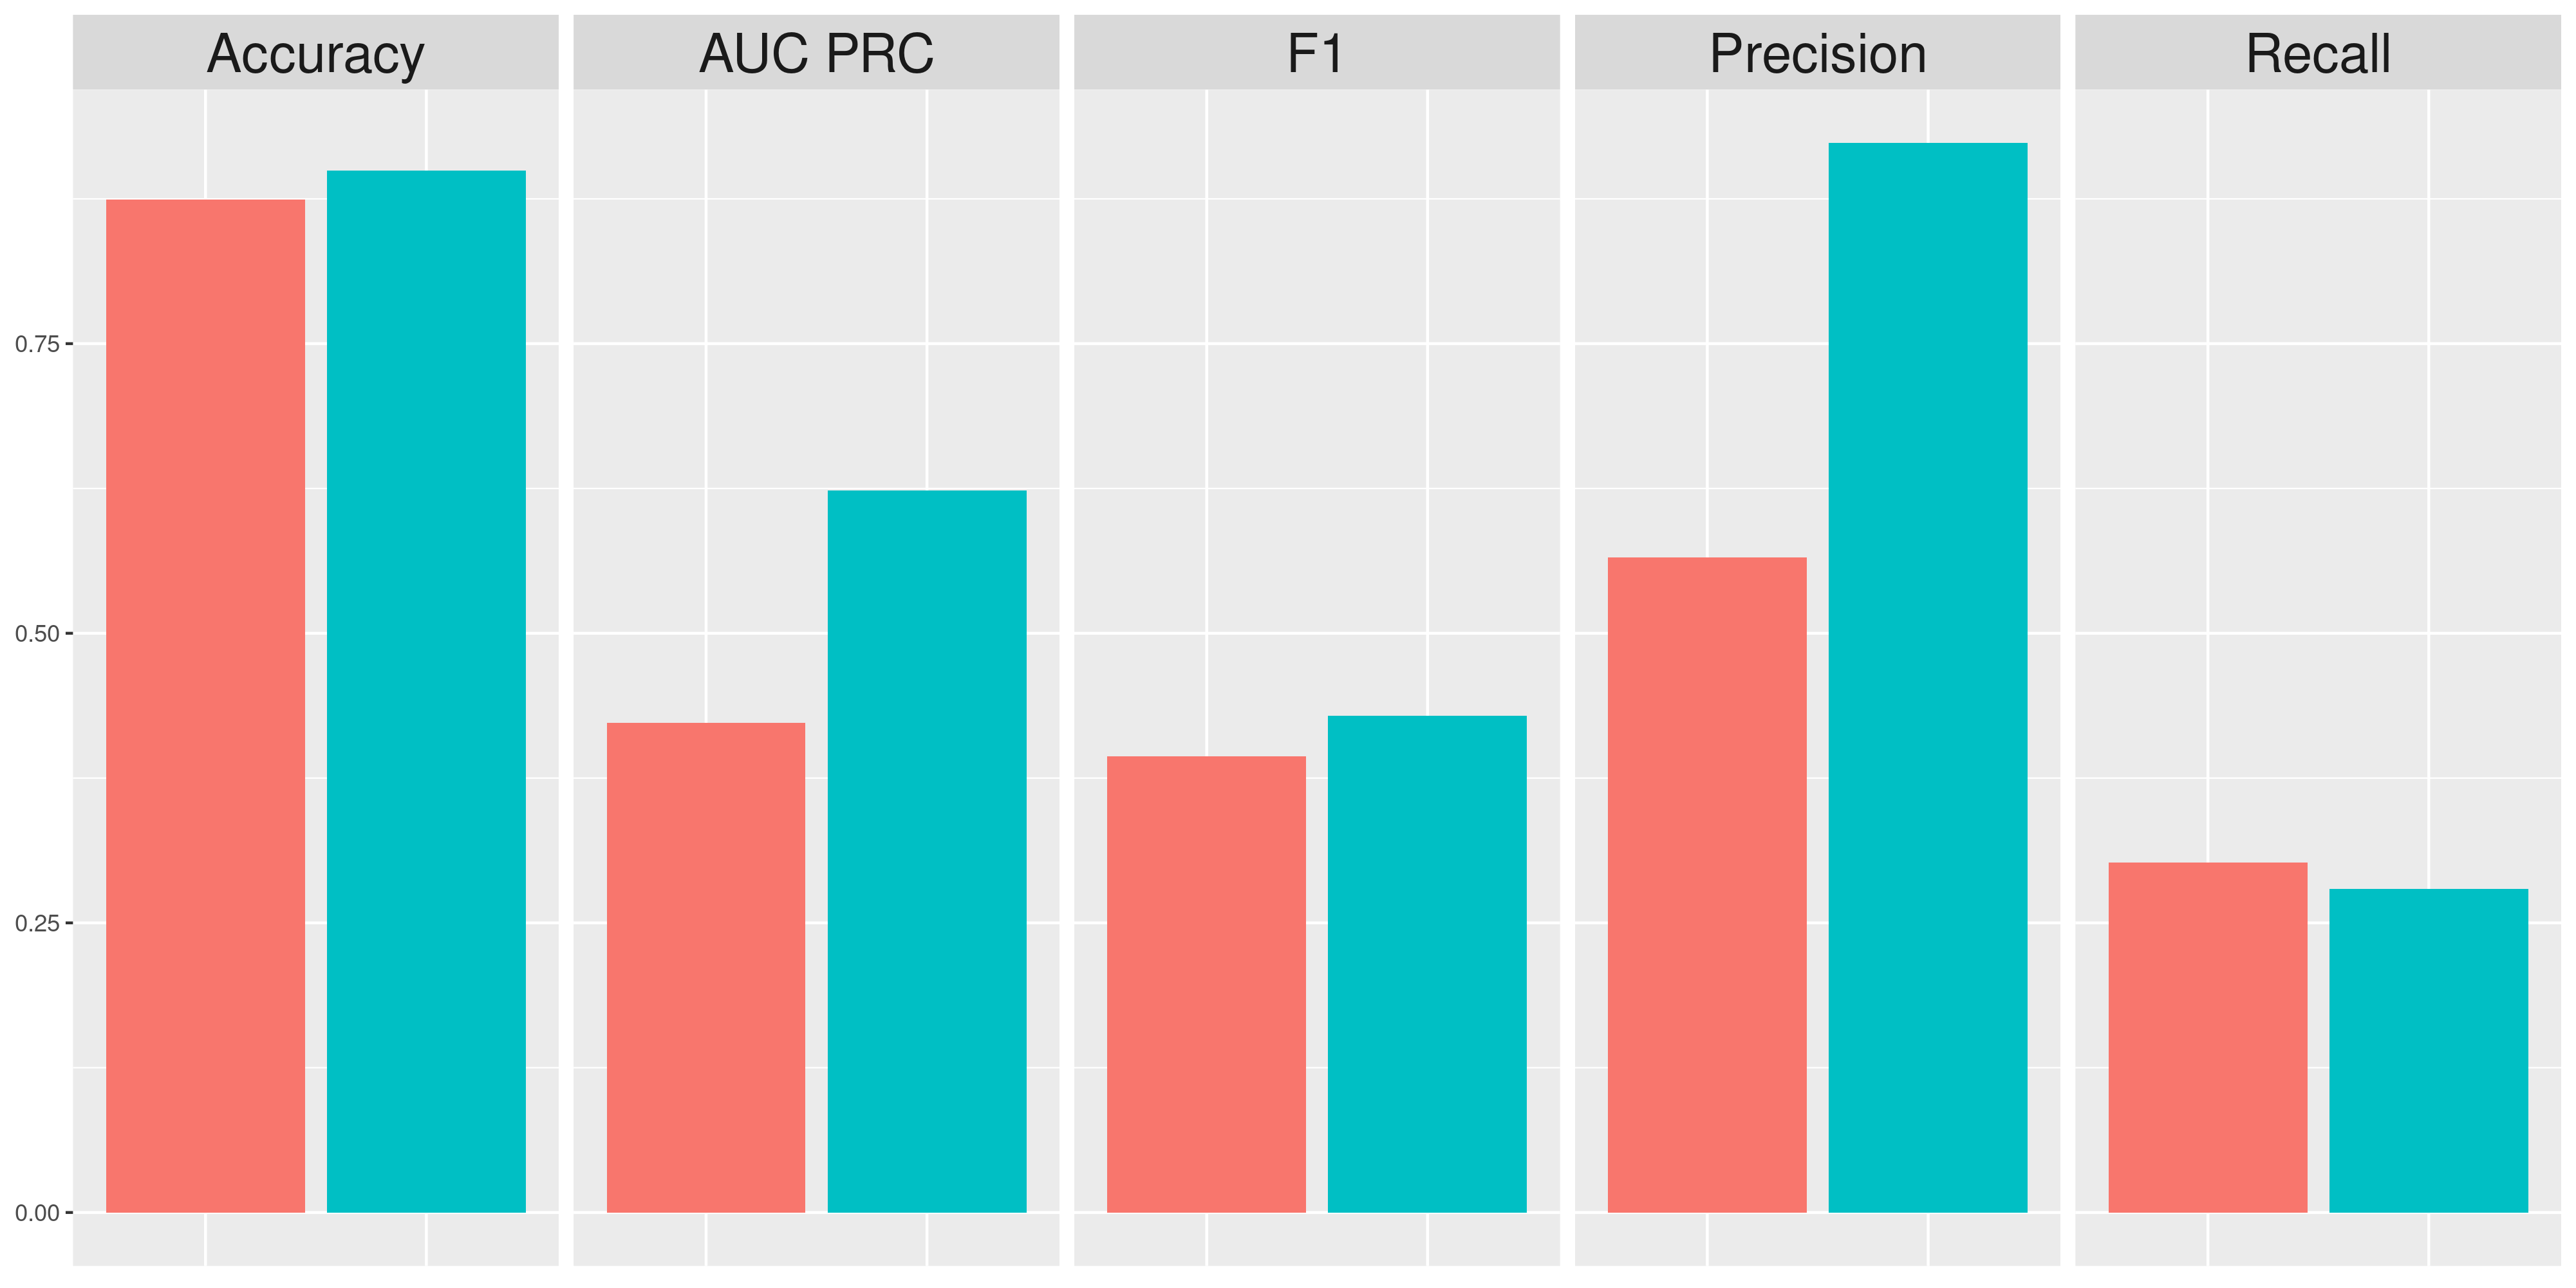
\includegraphics[width=12cm, height=8cm, keepaspectratio]{images/comparison/no-outliers/z-score_measures.png}
    }
    \quad
    \subfloat[Standardizzazione + PCA]{%
        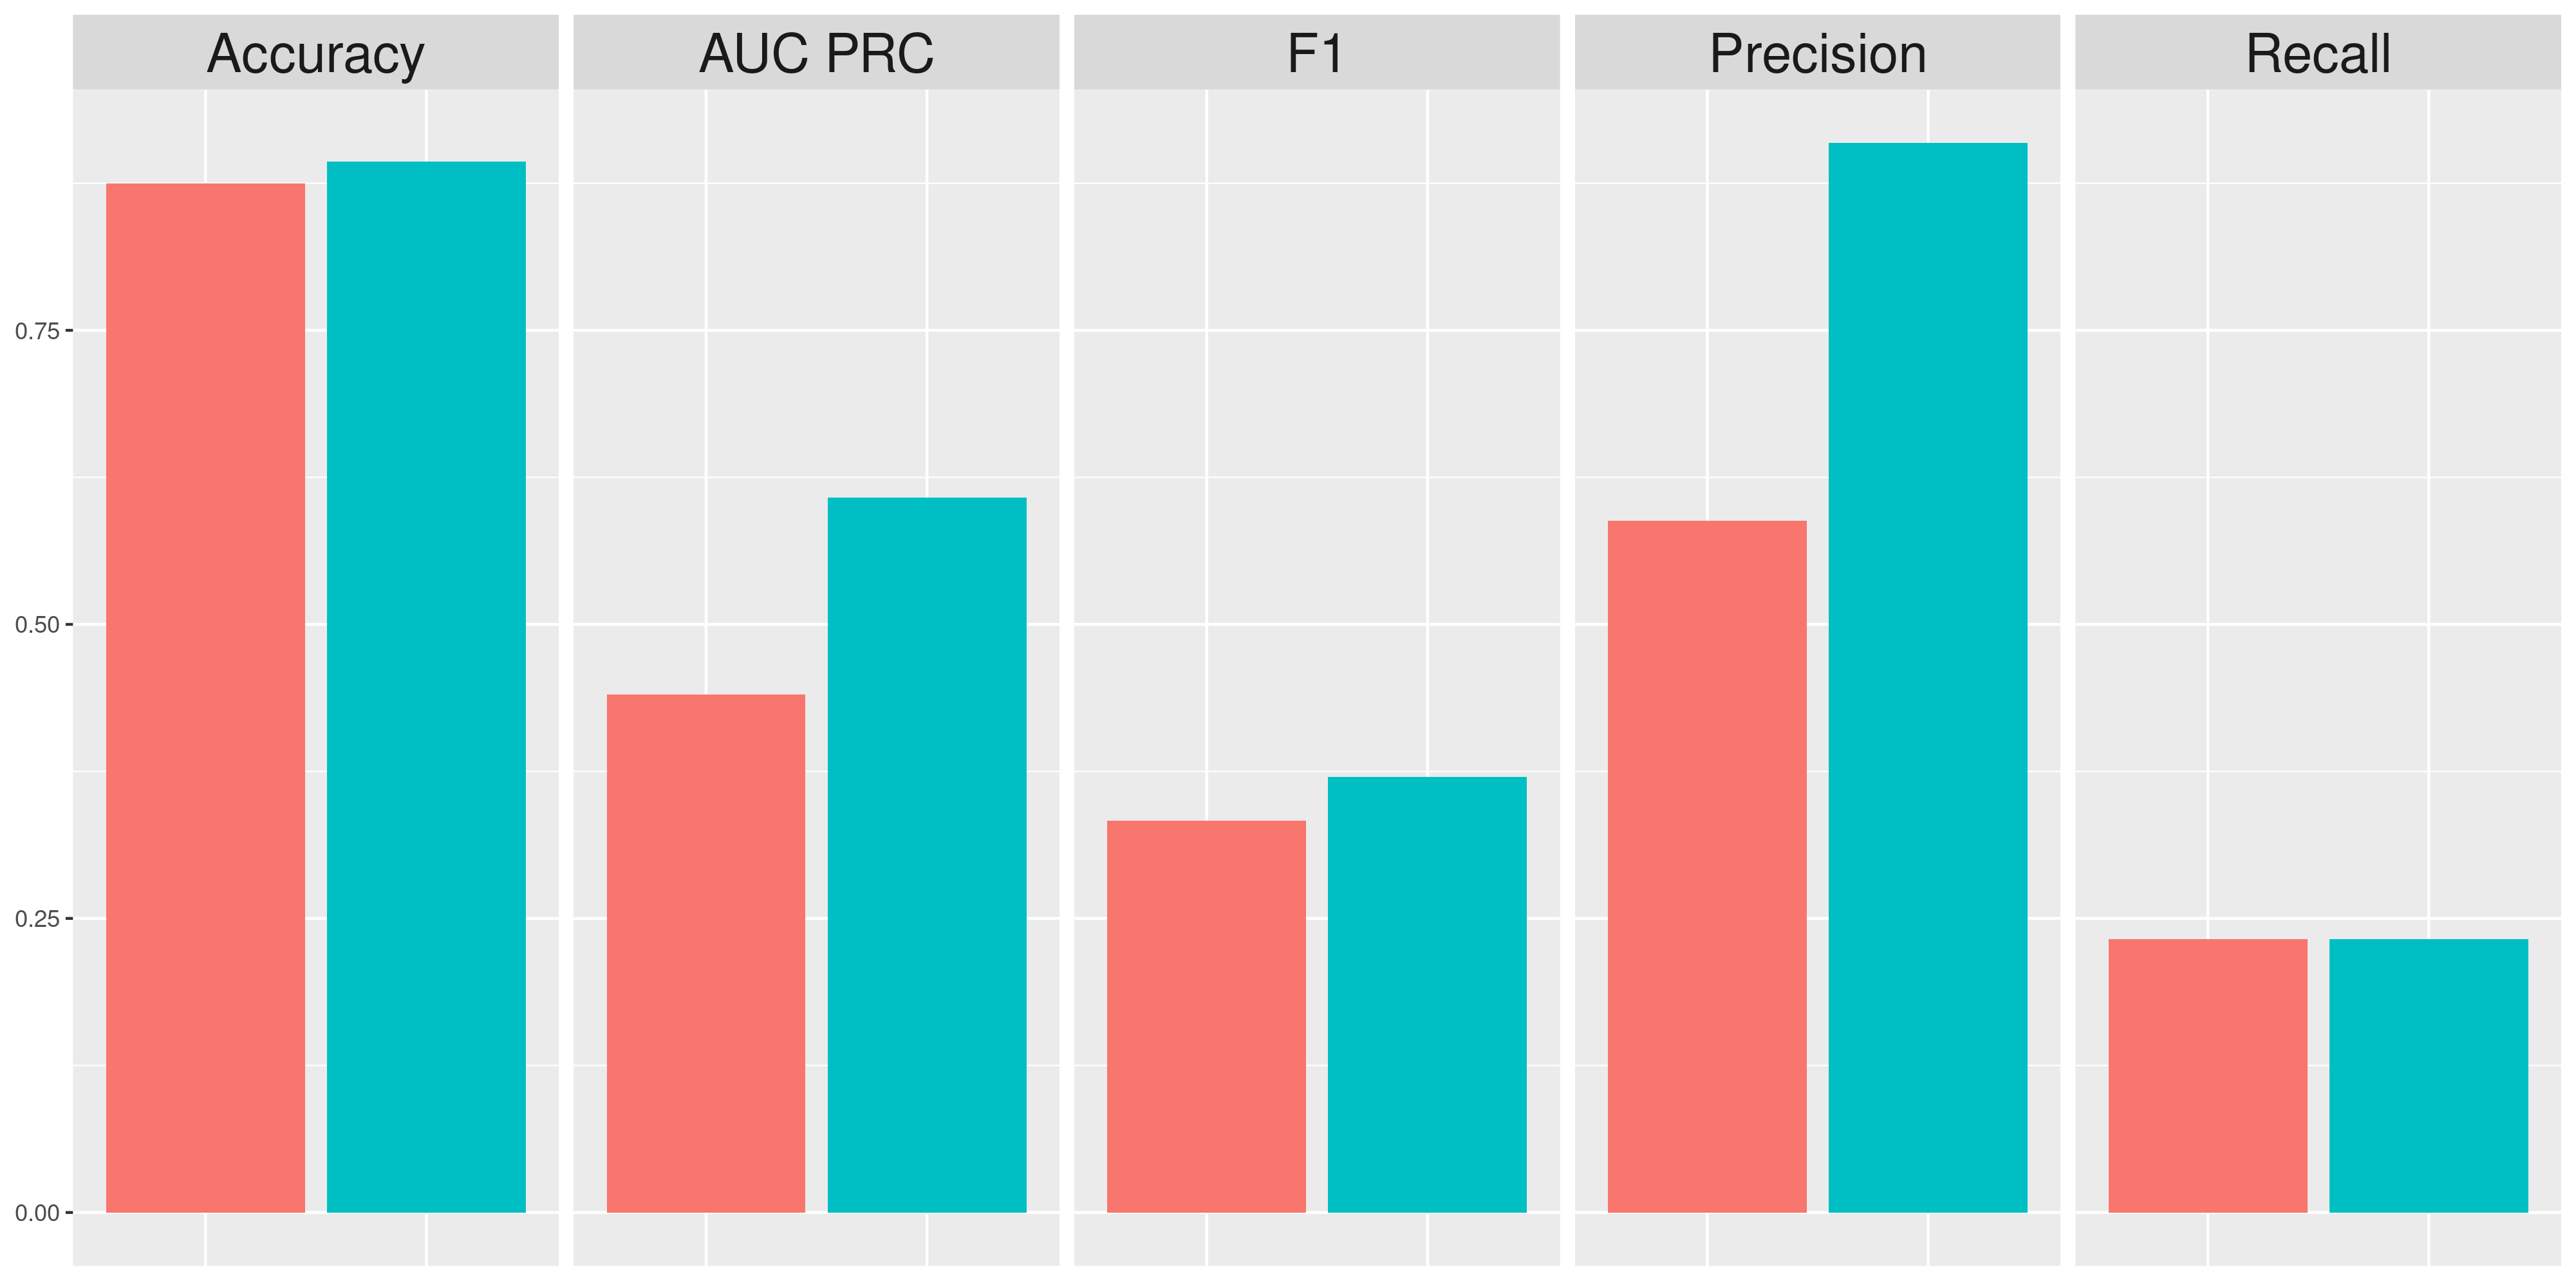
\includegraphics[width=12cm, height=8cm, keepaspectratio]{images/comparison/no-outliers/pca_measures.png}
    }
    
    \label{fig:measures_svm}
    \caption{Risultati dei due modelli (cart: rosso, radiale: blu) sul testset senza outliers}
\end{figure}


\noindent
Osservando le curve ROC e PRC possiamo notare come quelle dell'SVM radiale siano sempre superiori a quelle di CART.
Si riconferma che la rimozione degli outliers peggiora i risultati.
Dal caso [\ref{fig:a-roc}] non è possibile distinguere i risultati dalla curva PRC, per questo sono stati riportati in tabelle i valori di AUC (Area Under The Curve) che confermano che anche in questo caso l'SVM radiale raggiunge risultati migliori.

\newpage

\begin{figure}[H]
    \centering

    \subfloat[Standardizzazione]{%
        \label{fig:a-roc}
        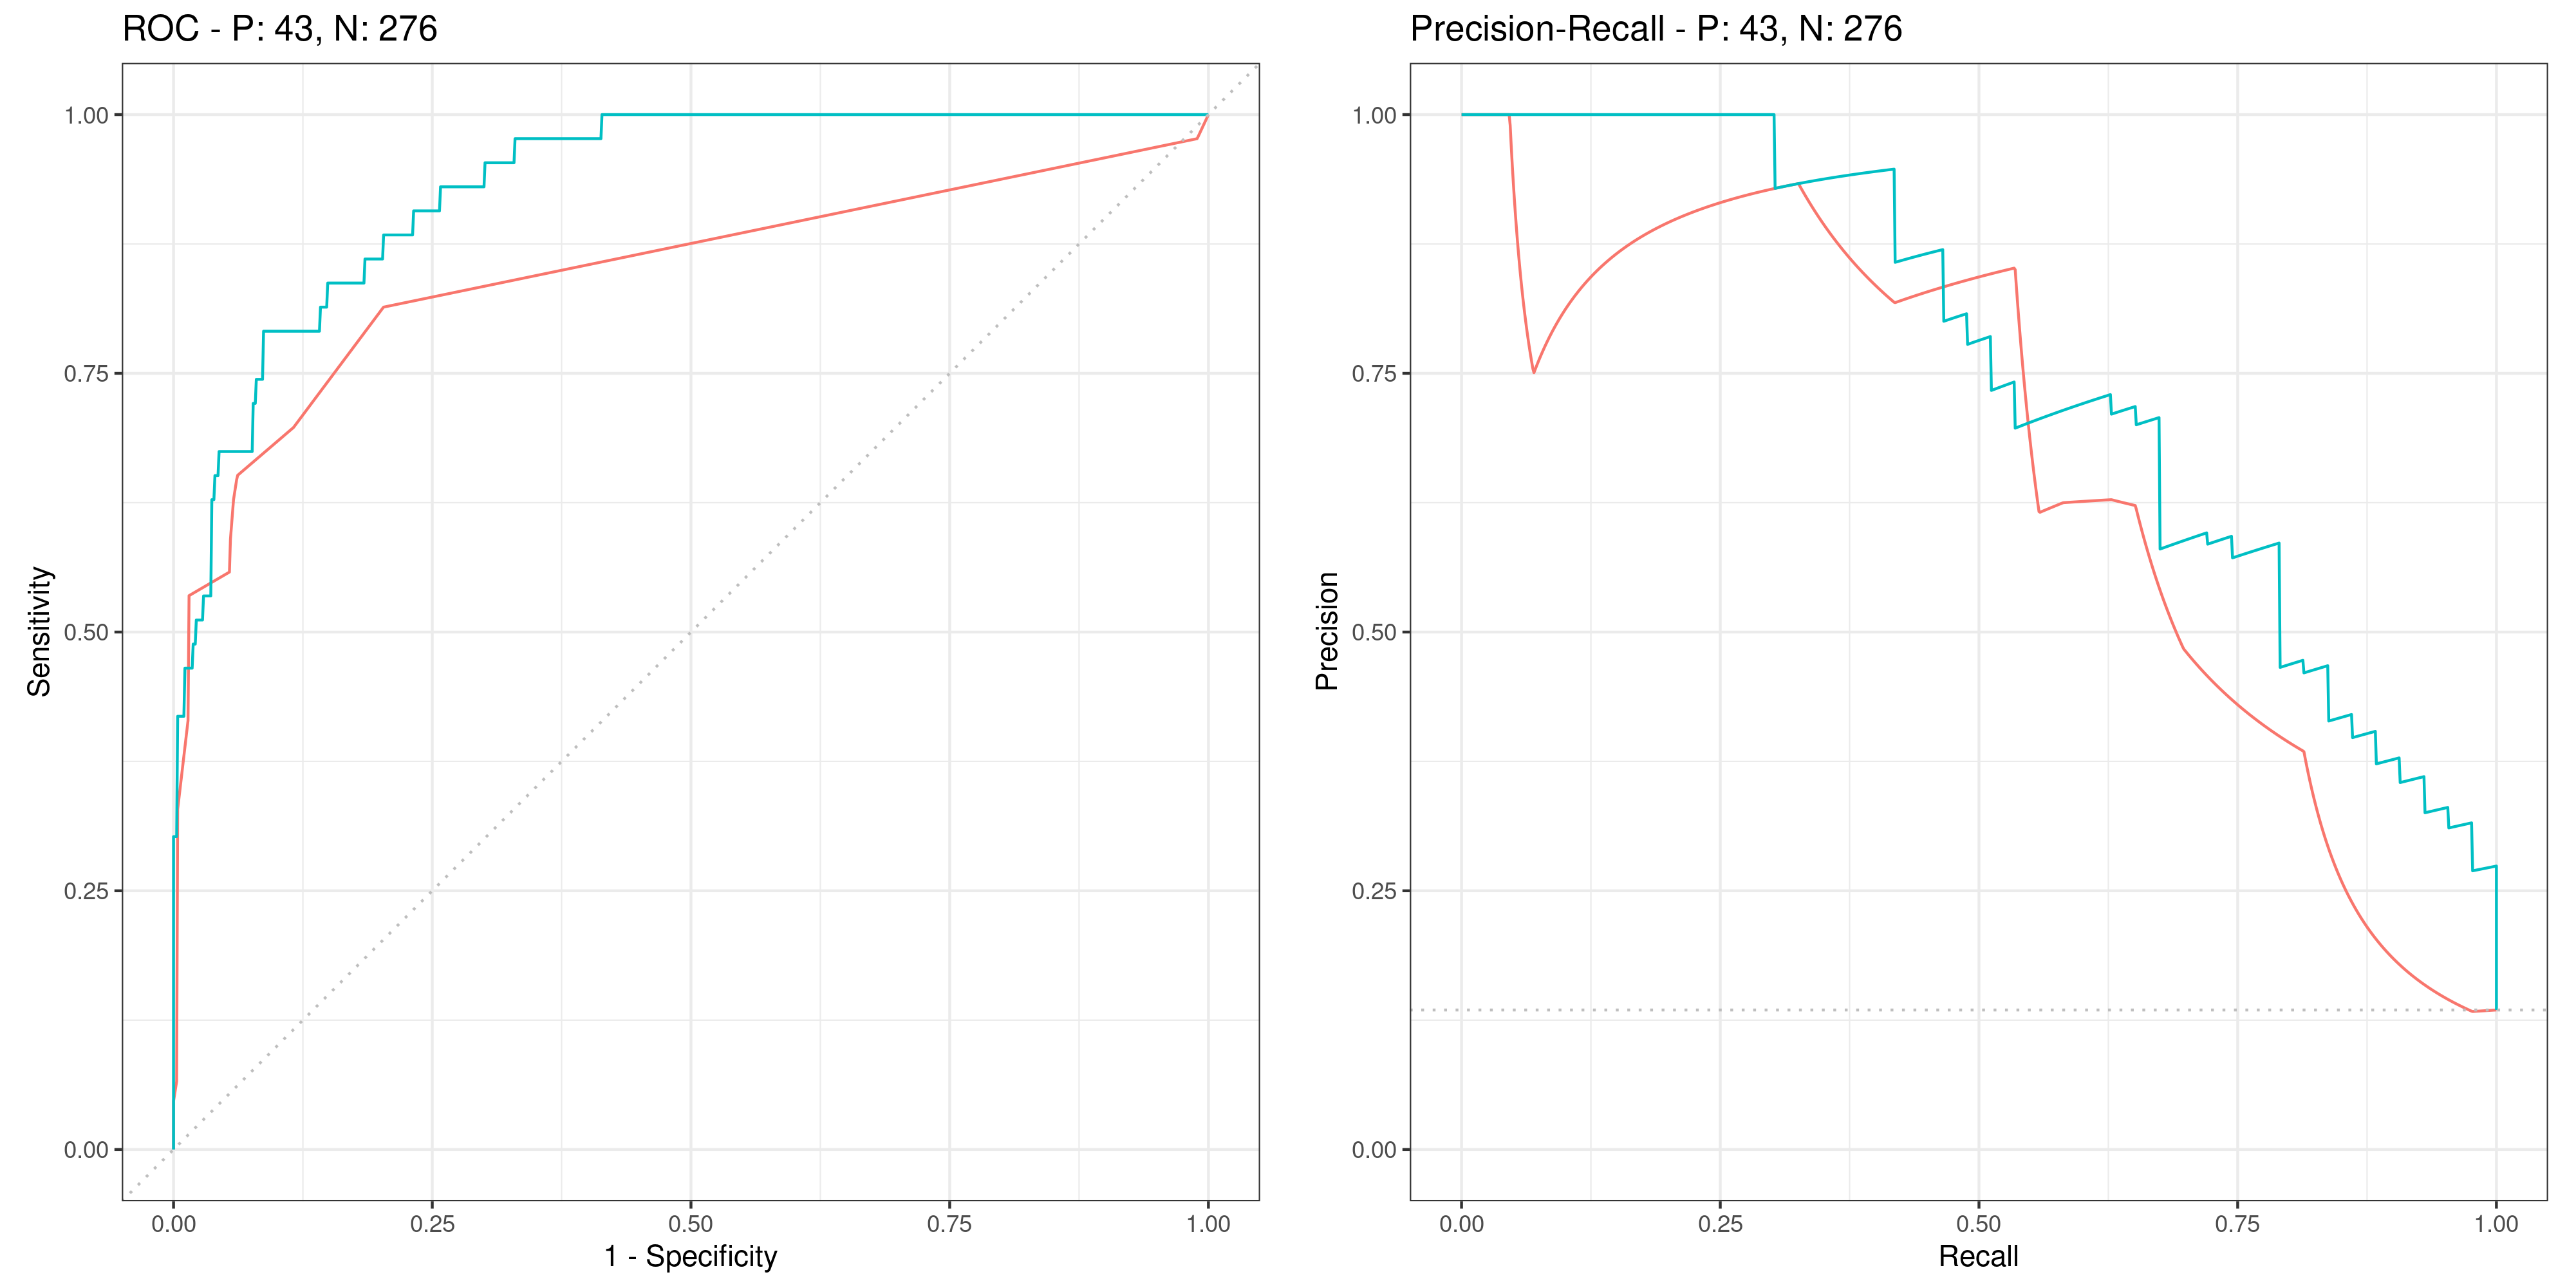
\includegraphics[width=\linewidth]{images/roc/outliers/z-score.png}
    }
    
    \quad
    
    \subfloat[Standardizzazione + PCA]{%
        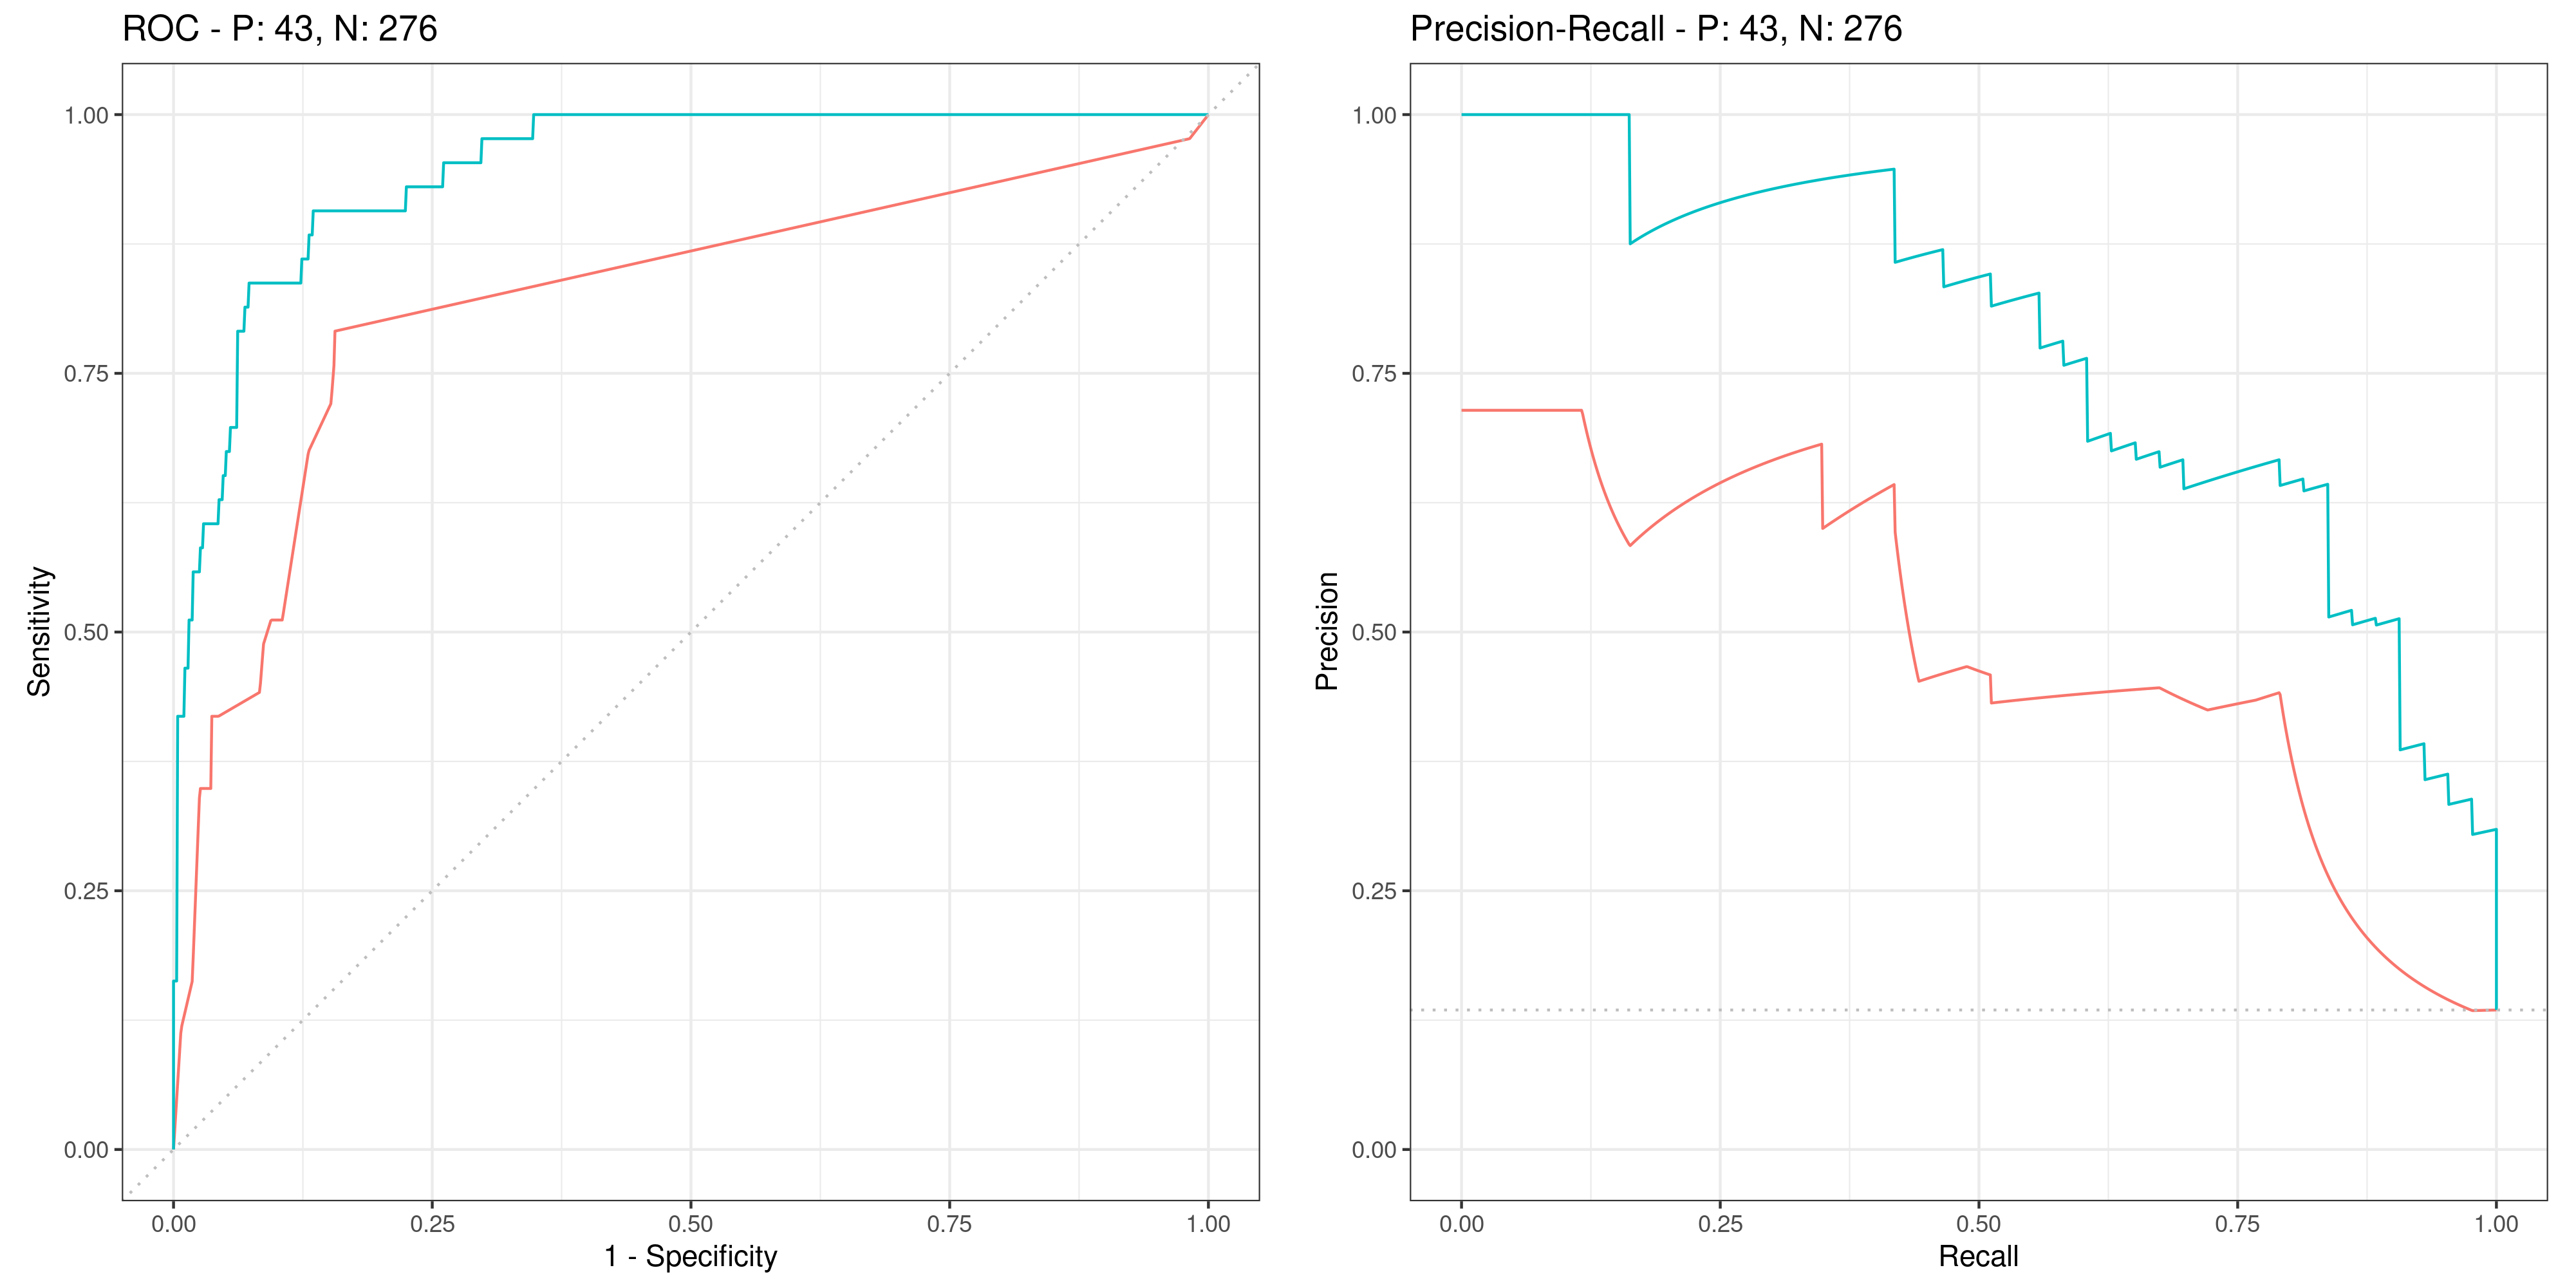
\includegraphics[width=\linewidth]{images/roc/outliers/pca.png}
    }

    \label{fig:roc_prc_svm_outliers}
    \caption{Curve ROC e PRC per i due modelli (cart: rosso, radiale: blu) sul testset con outliers}
\end{figure}

\begin{figure}[H]
    \centering

    \subfloat[Standardizzazione]{%
        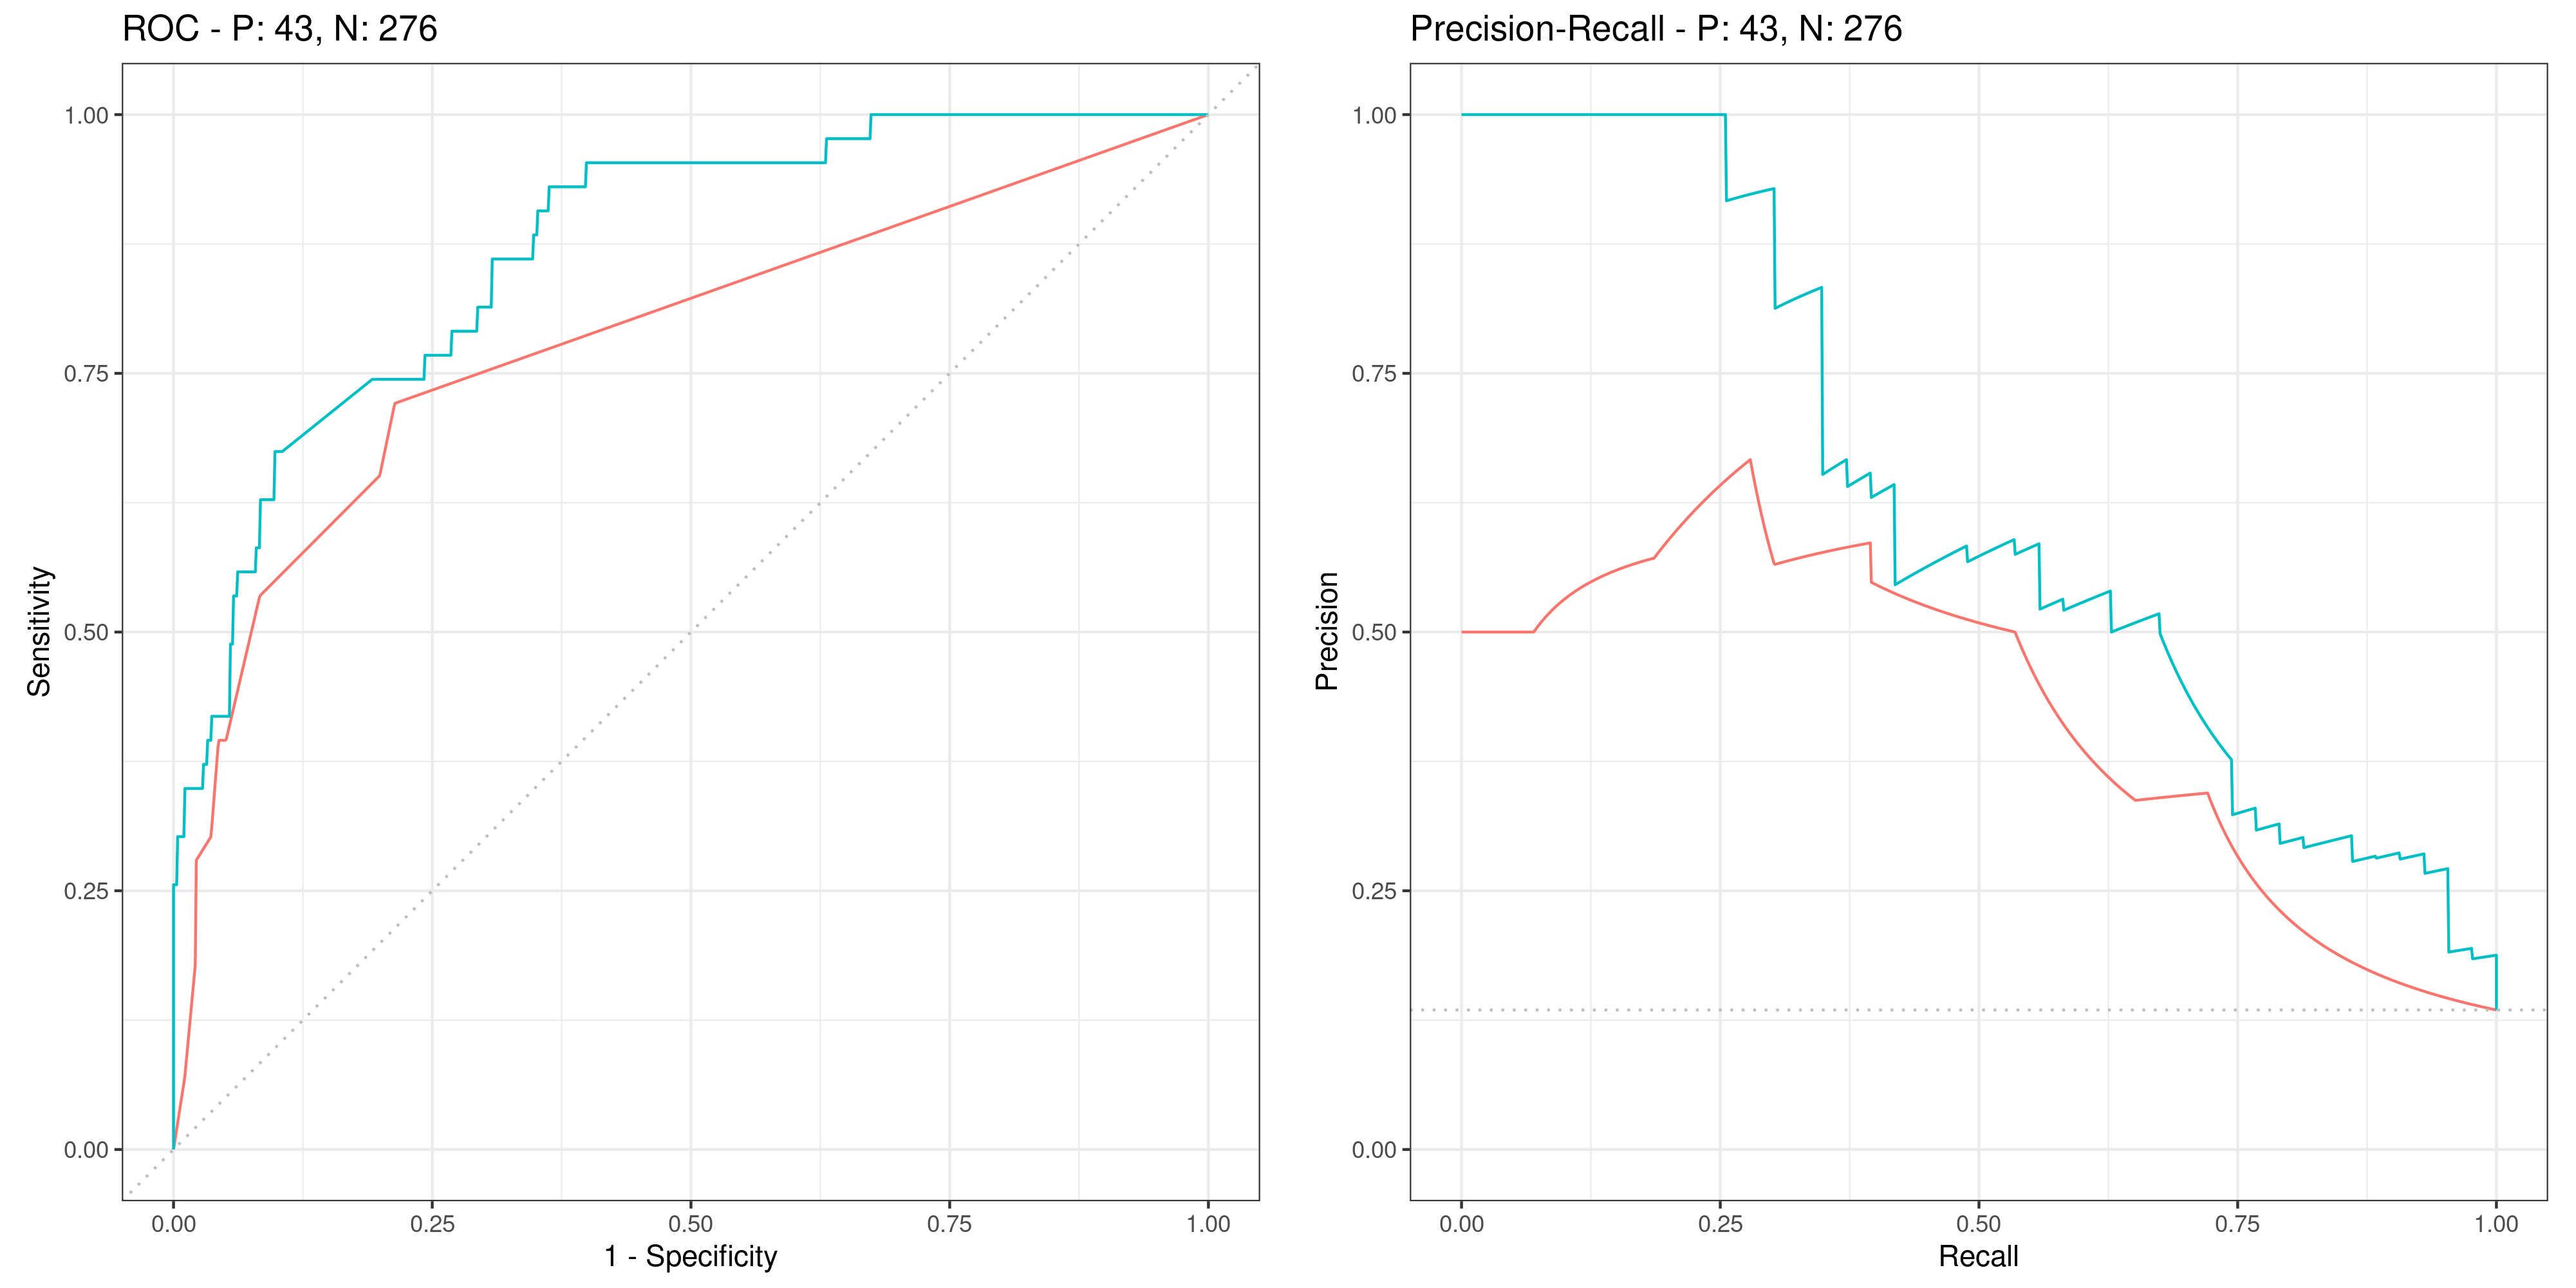
\includegraphics[width=\linewidth]{images/roc/no-outliers/z-score.png}
    }
    
    \quad
    
    \subfloat[Standardizzazione + PCA]{%
        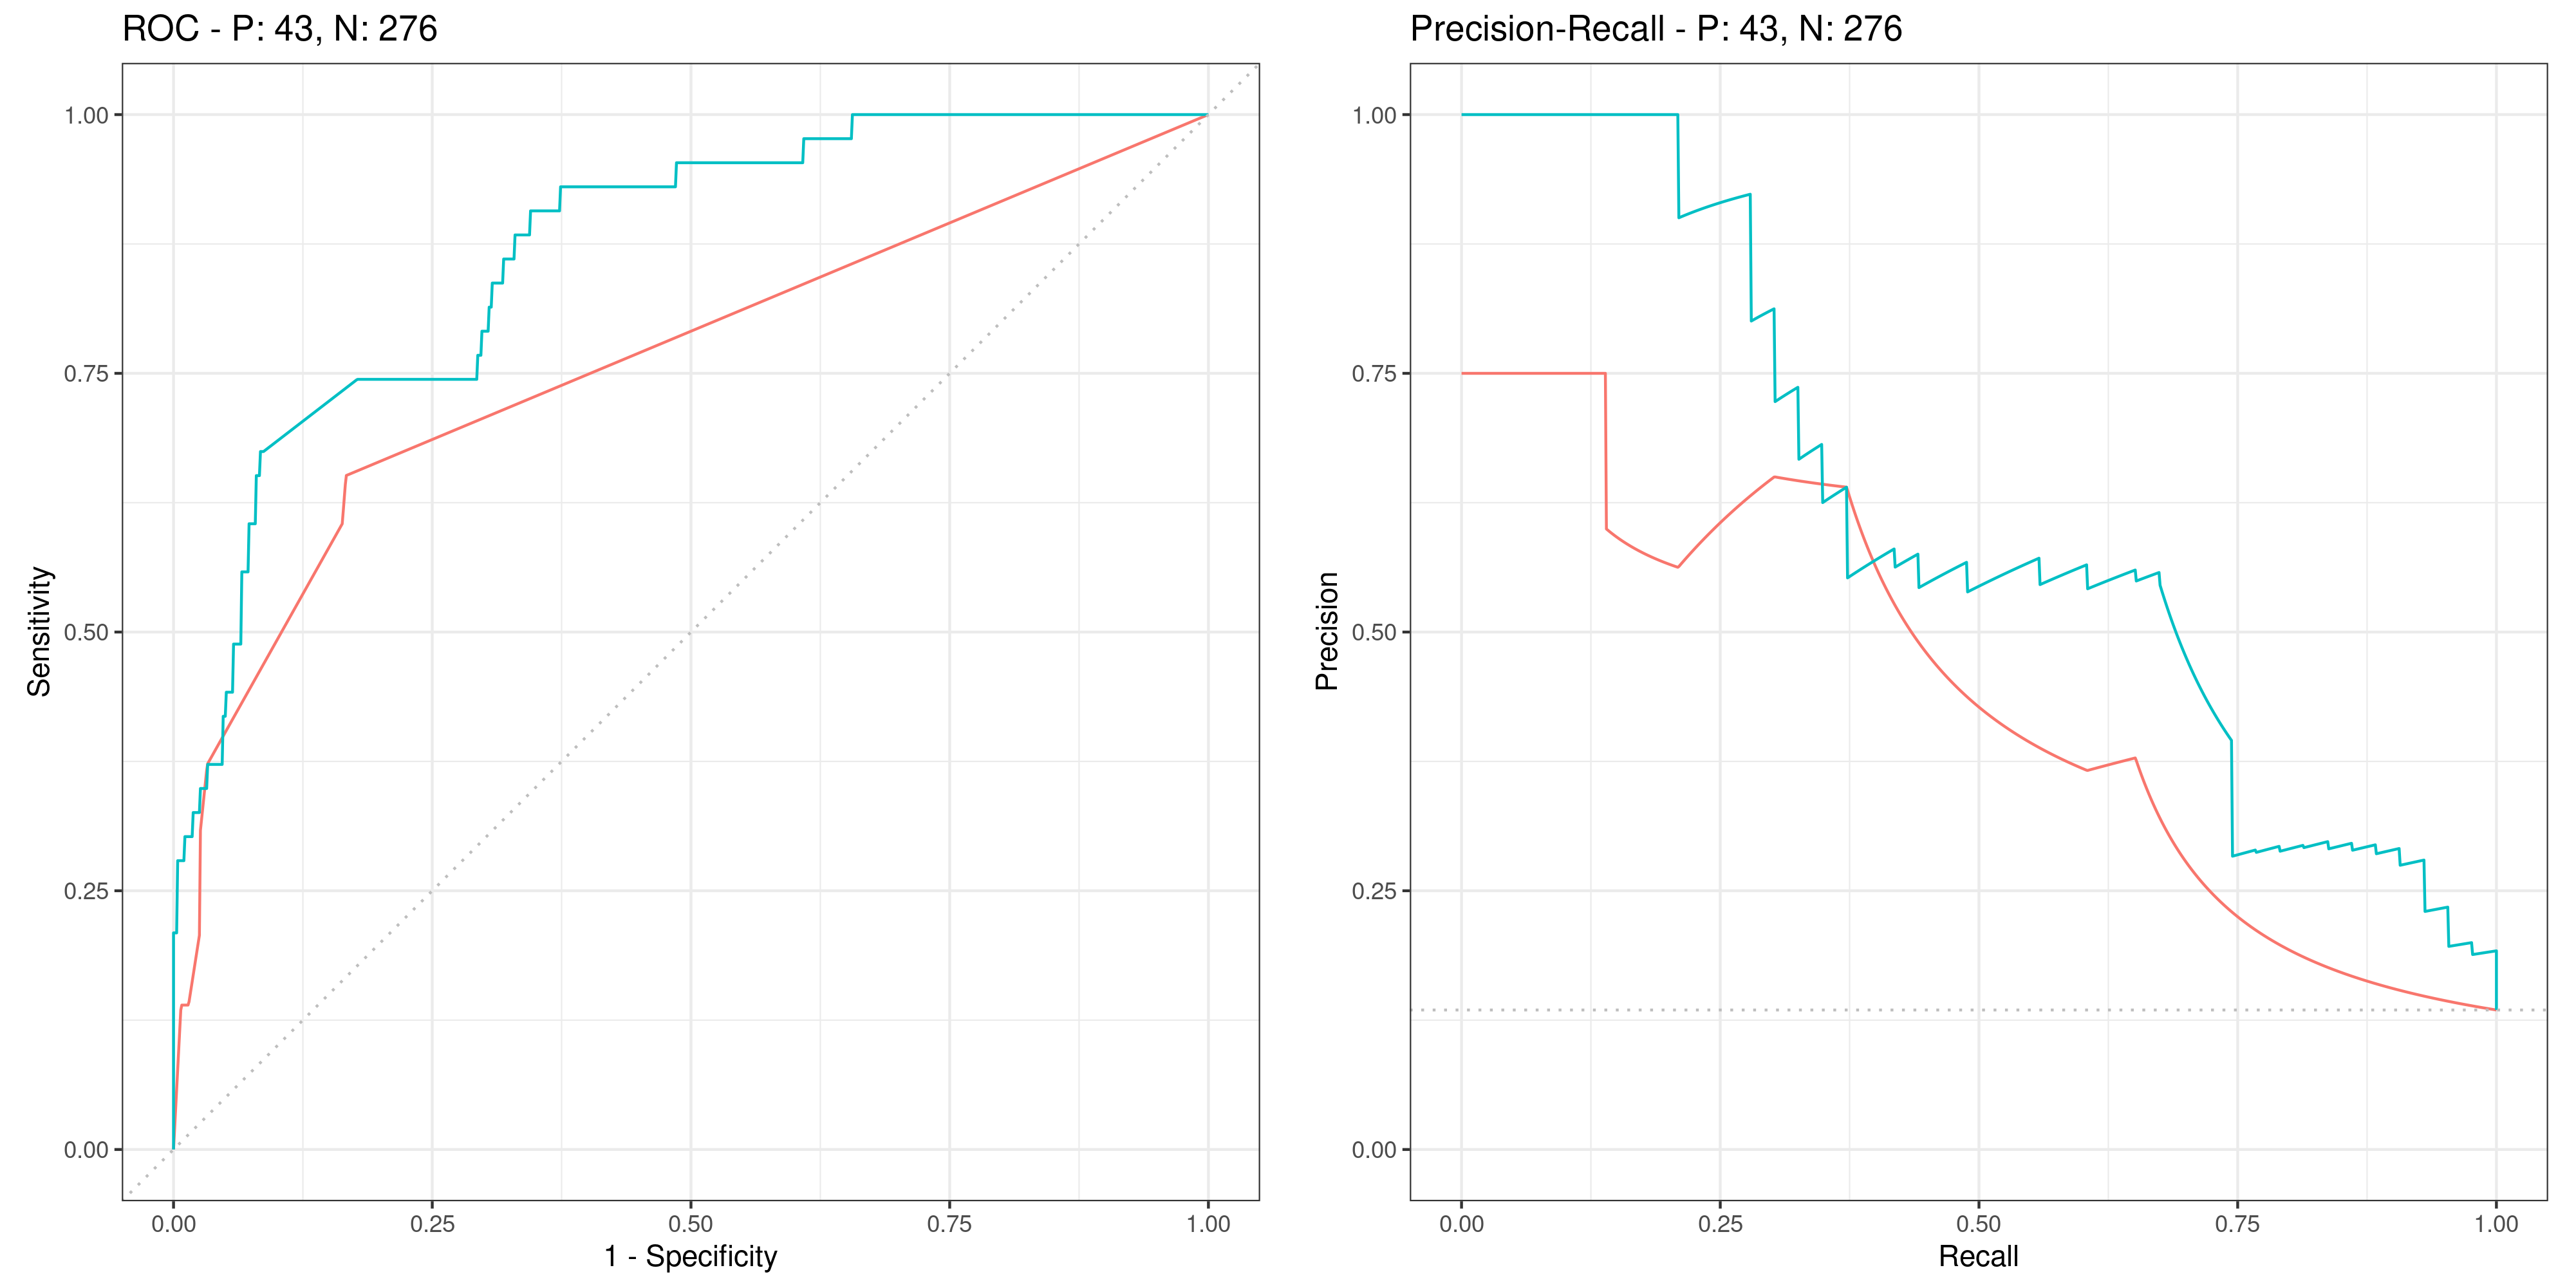
\includegraphics[width=\linewidth]{images/roc/no-outliers/pca.png}
    }

     \label{fig:roc_prc_svm}
    \caption{Curve ROC e PRC per i due modelli (cart: rosso, radiale: blu) sul testset senza outliers}
\end{figure}

\newpage

\noindent
Riassumiamo nuovamente i risultati presentati nelle tabelle sottostanti. Per scegliere i modelli migliori che verranno proposti in questo lavoro, è necessario analizzare le differenze tra Standardizzazione + PCA e Standardizzazione nel caso in cui gli outliers vengono mantenuti.
CART con Standardizzazione ha risultati migliori della controparte con Standardizzazione + PCA.
L'SVM radiale con Standardizzazione + PCA è leggermente migliore rispetto alla controparte con Standardizzazione.

\begin{table}[H]
\centering
\resizebox{\textwidth}{!}{%
\begin{tabular}{@{}ccccccccc@{}}
\toprule
\textbf{Models} & \textbf{Overall Accuracy} & \textbf{Precision} & \textbf{Recall} & \textbf{F1} & \textbf{ROC AUC} & \textbf{PRC AUC} & \textbf{95\% CI} & \textbf{P-Value} \\ \midrule
cart & 0.9154 & 0.83333 & \textbf{0.46512} & \textbf{0.59701} & 0.8476154 & 0.6564769 & (0.8792, 0.9435) & 0.003747 \\
svm & \textbf{0.9122} & \textbf{0.94118} & 0.37209 & 0.53333 & \textbf{0.9313279} & \textbf{0.7520759} & (0.8756, 0.9409) & 0.006404 \\ \bottomrule
\end{tabular}%
}
\caption{Risultati modelli scelti con Standardizzazione}
\label{tab:my-table}
\end{table}

\begin{table}[H]
\centering
\resizebox{\textwidth}{!}{%
\begin{tabular}{@{}ccccccccc@{}}
\toprule
\textbf{Models} & \textbf{Overall Accuracy} & \textbf{Precision} & \textbf{Recall} & \textbf{F1} & \textbf{ROC AUC} & \textbf{PRC AUC} & \textbf{95\% CI} & \textbf{P-Value} \\ \midrule
cart & 0.884 & 0.6 & \textbf{0.4186} & 0.49315 & 0.8194725 & 0.485855 & (0.8437, 0.917) & 0.18452 \\
svm & \textbf{0.9122} & \textbf{0.94118} & 0.37209 & \textbf{0.53333} & \textbf{0.9469161} & \textbf{0.7732596} & (0.8756, 0.9409) & 0.006404 \\ \bottomrule
\end{tabular}%
}
\caption{Risultati modelli scelti con Standardizzazione + PCA}
\label{tab:my-table}
\end{table}

\begin{table}[H]
\centering
\resizebox{\textwidth}{!}{%
\begin{tabular}{@{}ccccccccc@{}}
\toprule
\textbf{Models} & \textbf{Overall Accuracy} & \textbf{Precision} & \textbf{Recall} & \textbf{F1} & \textbf{ROC AUC} & \textbf{PRC AUC} & \textbf{95\% CI} & \textbf{P-Value} \\ \midrule
cart & 0.8746 & 0.56522 & \textbf{0.30233} & 0.39394 & 0.7817661 & 0.4226265 & (0.8332, 0.9089) & 0.347156 \\
svm & \textbf{0.8997} & \textbf{0.92308} & 0.27907 & \textbf{0.42857} & \textbf{0.8711662} & \textbf{0.6230968} & (0.8613, 0.9304) & 0.03864 \\ \bottomrule
\end{tabular}%
}
\caption{Risultati modelli scelti con Standardizzazione e rimozione outliers}
\label{tab:my-table}
\end{table}

\begin{table}[H]
\centering
\resizebox{\textwidth}{!}{%
\begin{tabular}{@{}ccccccccc@{}}
\toprule
\textbf{Models} & \textbf{Overall Accuracy} & \textbf{Precision} & \textbf{Recall} & \textbf{F1} & \textbf{ROC AUC} & \textbf{PRC AUC} & \textbf{95\% CI} & \textbf{P-Value} \\ \midrule
cart & 0.8746 & 0.58824 & \textbf{0.23256} & 0.33333 & 0.7598163 & 0.440484 & (0.8332, 0.9089) & 0.3472 \\
svm & \textbf{0.8934} & \textbf{0.90909} & \textbf{0.23256} & \textbf{0.37037} & \textbf{0.8684277} & \textbf{0.6079154} & (0.8543, 0.9251) & 0.07852 \\ \bottomrule
\end{tabular}%
}
\caption{Risultati modelli scelti con Standardizzazione + PCA e rimozione outliers}
\label{tab:my-table}
\end{table}

\noindent
Concludiamo che i modelli migliori sono CART con Standardizzazione e SVM radiale con Standardizzazione + PCA, entrambi mantenendo gli outliers.

\newpage

\section{Confronto fra i modelli scelti}
In questa sezione andiamo a confrontare i due modelli proposti per la trattazione del nostro problema.

\noindent
Mostriamo ora le matrici di confusione dei modelli testati sul testset composto da 319 istanze di cui 276 positive e 43 negative.
Dalle matrici di confusione possiamo vedere che i modelli non sembrano così diversi e come entrambi soffrono dello sbilanciamento del dataset. Infatti i nostri modelli classificano correttamente quasi tutte le istanze appartenenti alla classe maggioritaria, mentre sbagliano molto di più sulla classe minoritaria.

\begin{figure}[H]
    \centering
    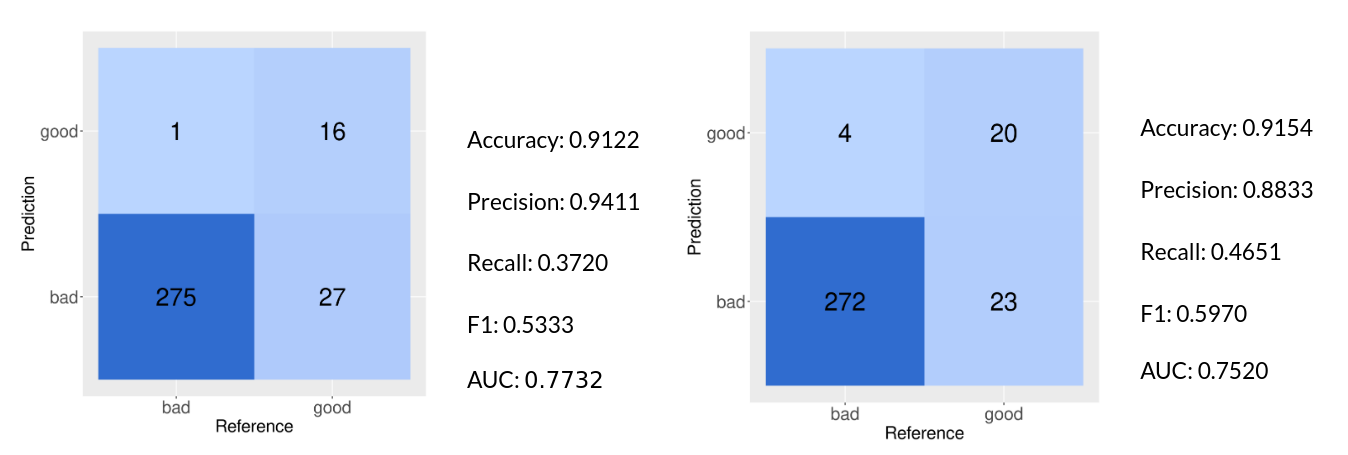
\includegraphics[width=\linewidth]{images/comparison/comparison2.png}
     \label{fig:confusion_matrix}
    \caption{Matrice di confusione sul testset per SVM Radiale con Standardizzazione + PCA (sinistra) e CART con Standardizzazione (destra)}
\end{figure}

\noindent
Comparando le metriche ottenute dai due modelli possiamo vedere come non ci sia una grossa differenza, tra alti valori di Precision e bassi valori di Recall, non considerando l'Accuracy come già detto precedente non è un buon indicatore. L'AUC è un indicatore migliore infatti notiamo che l'SVM radiale supera CART in AUC e Precision, mentre CART è migliore in Recall e F1.

\newpage

\noindent
Mostrando la ROC e la PRC è possibile vedere come l'SVM radiale superi CART in entrambe seppure di poco, rispettivamente 0.9469161/0.7732596 0.9313279/0.7520759.
\begin{figure}[H]
    \centering
    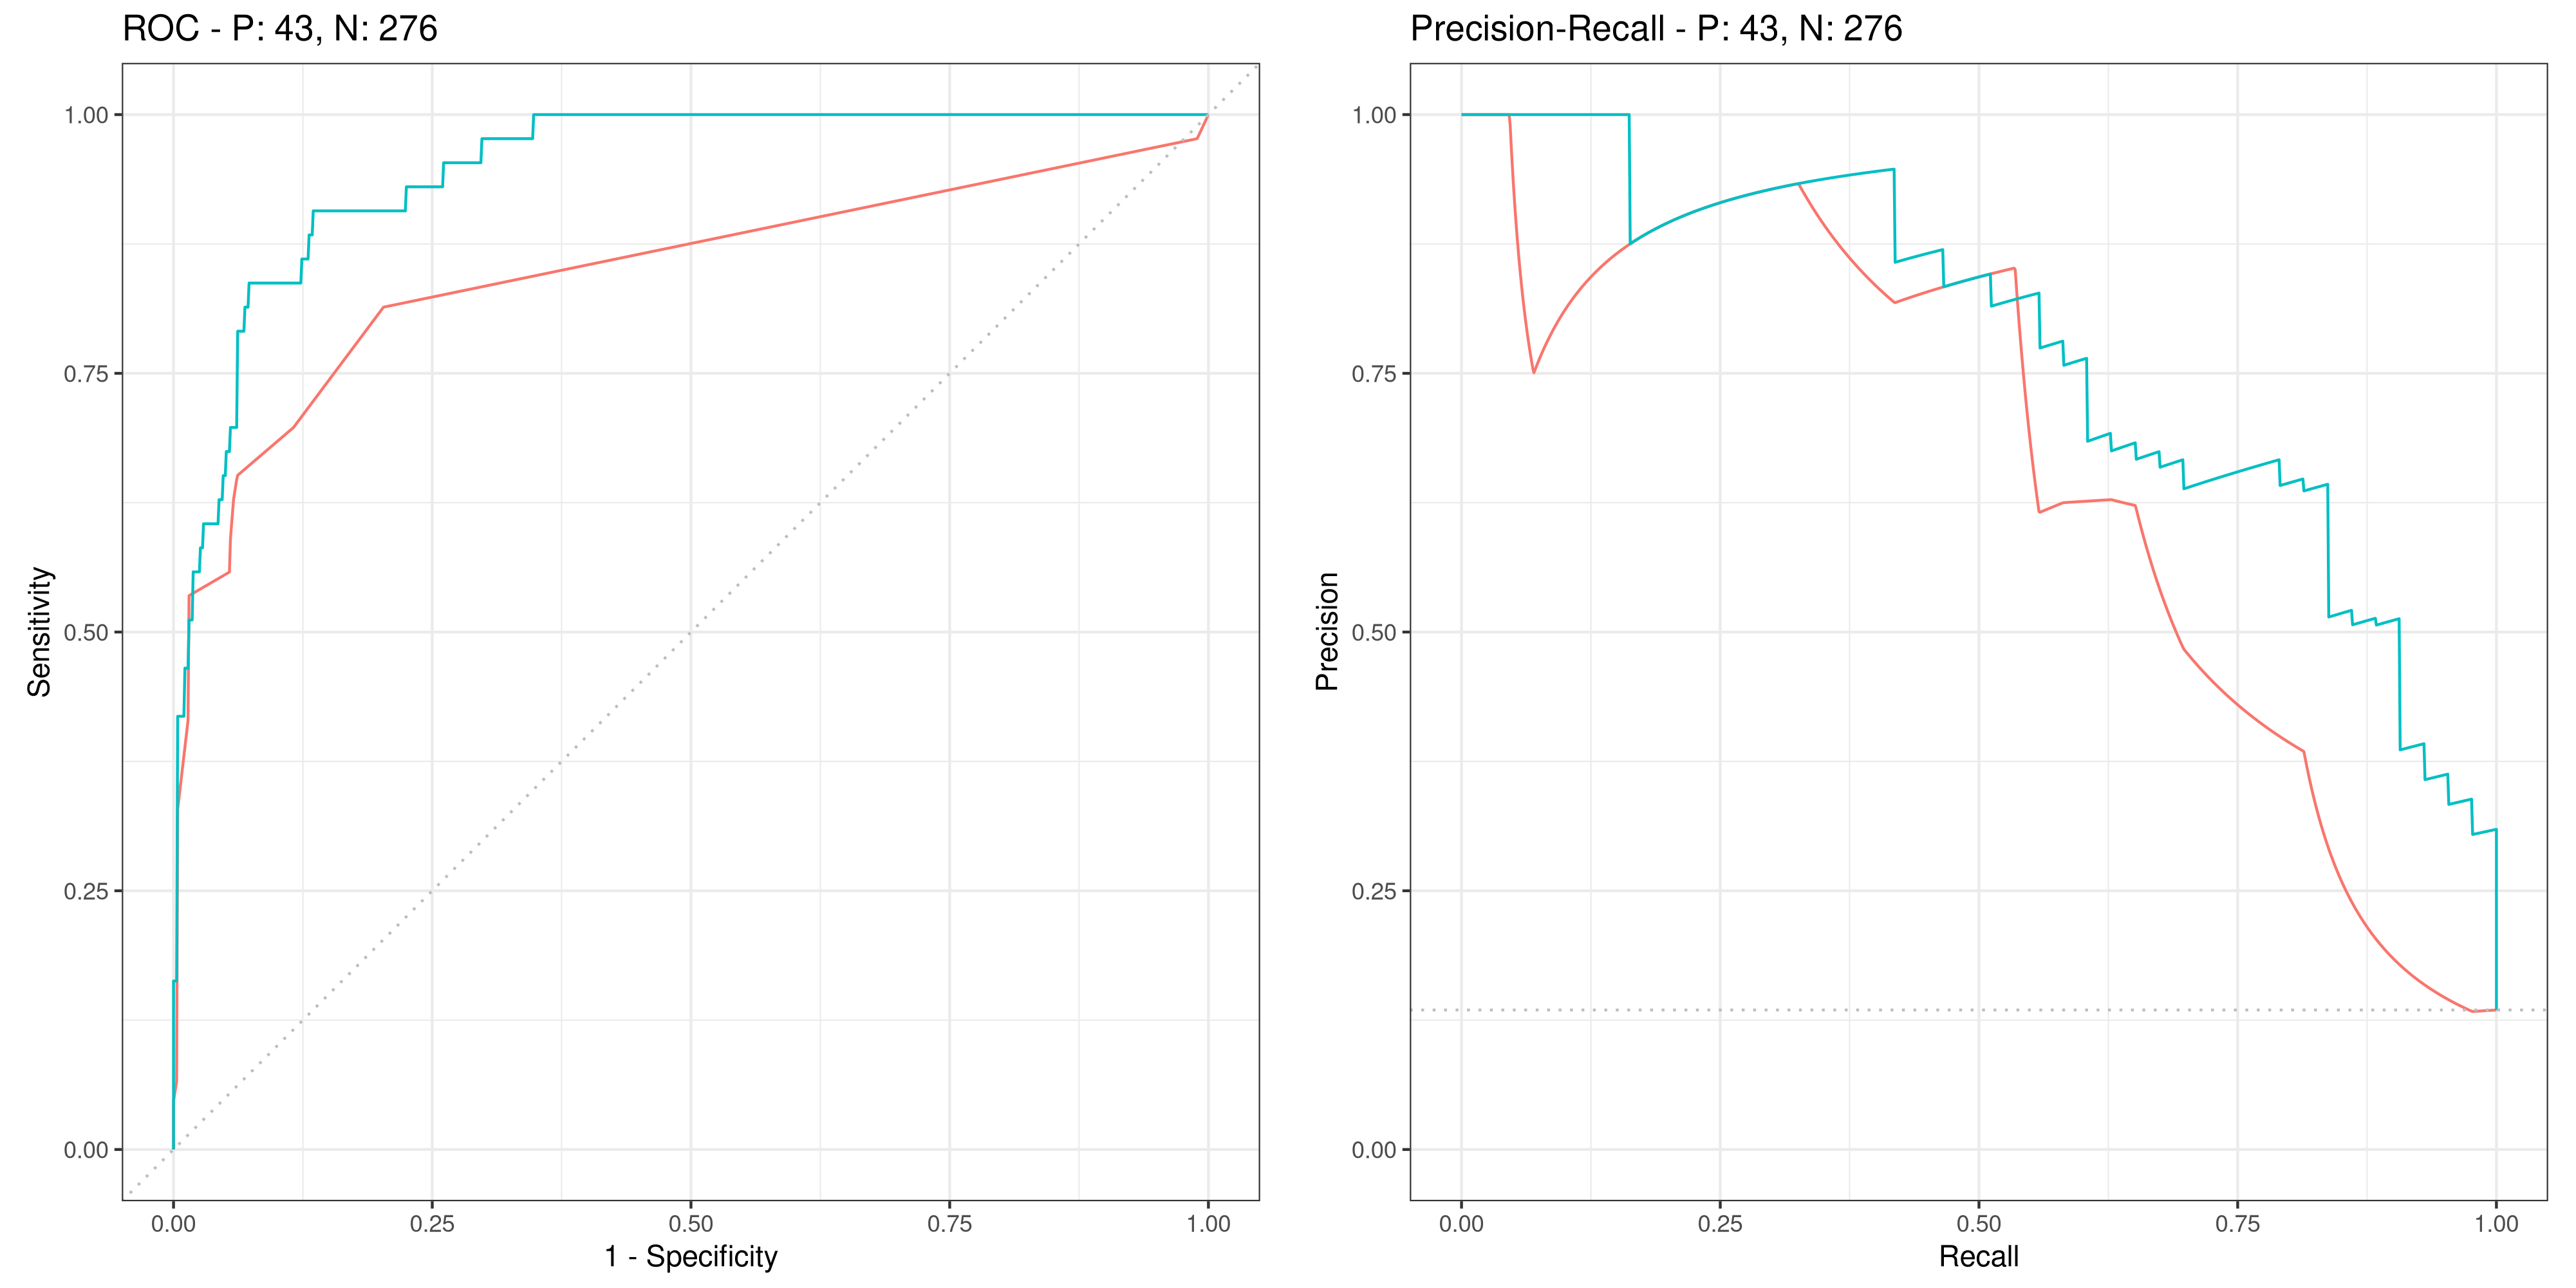
\includegraphics[width=\linewidth]{images/comparison/best/best_roc.png}
     \label{fig:roc_prc_modelli_proposti}
    \caption{Grafici ROC e PRC per i due modelli proposti, (cart: rosso, radiale: blu)}
\end{figure}

\begin{figure}[H]
    \centering
    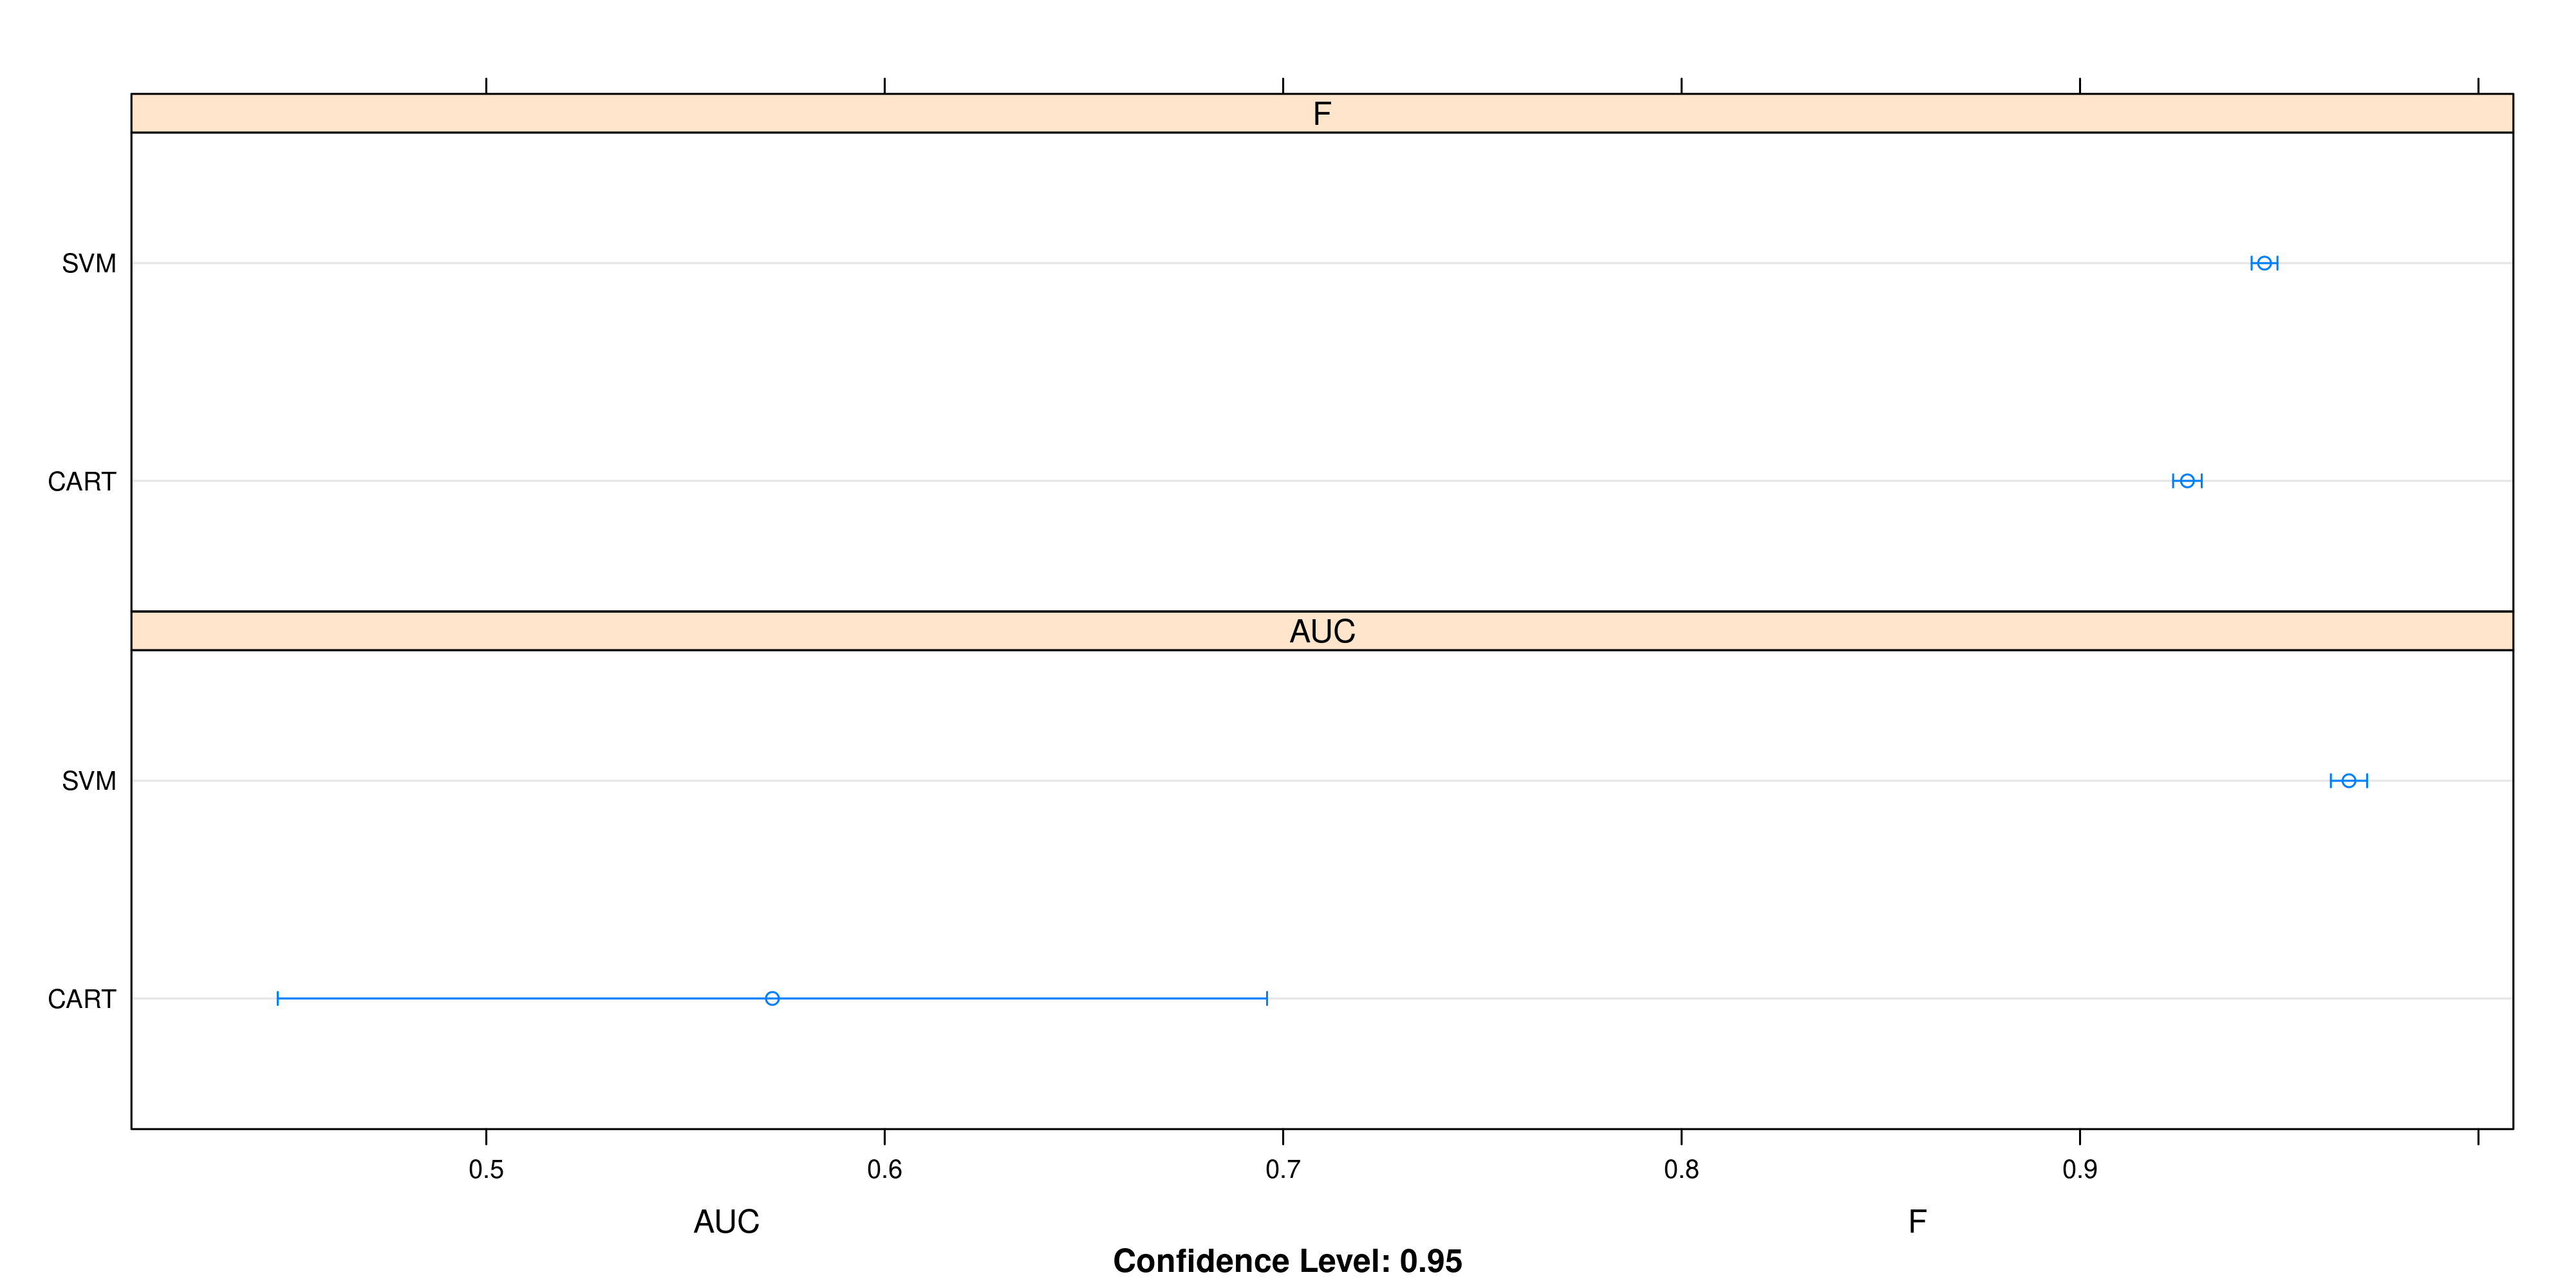
\includegraphics[width=\linewidth]{images/comparison/best/best_dotplot_af.png}
     \label{fig:ci1_modelli_proposti}
    \caption{Intervalli di confidenza dei modelli proposti per AUC e F1, (svmRadial: svm radiale, rpart2: cart)}
\end{figure}

\begin{figure}[H]
    \centering
    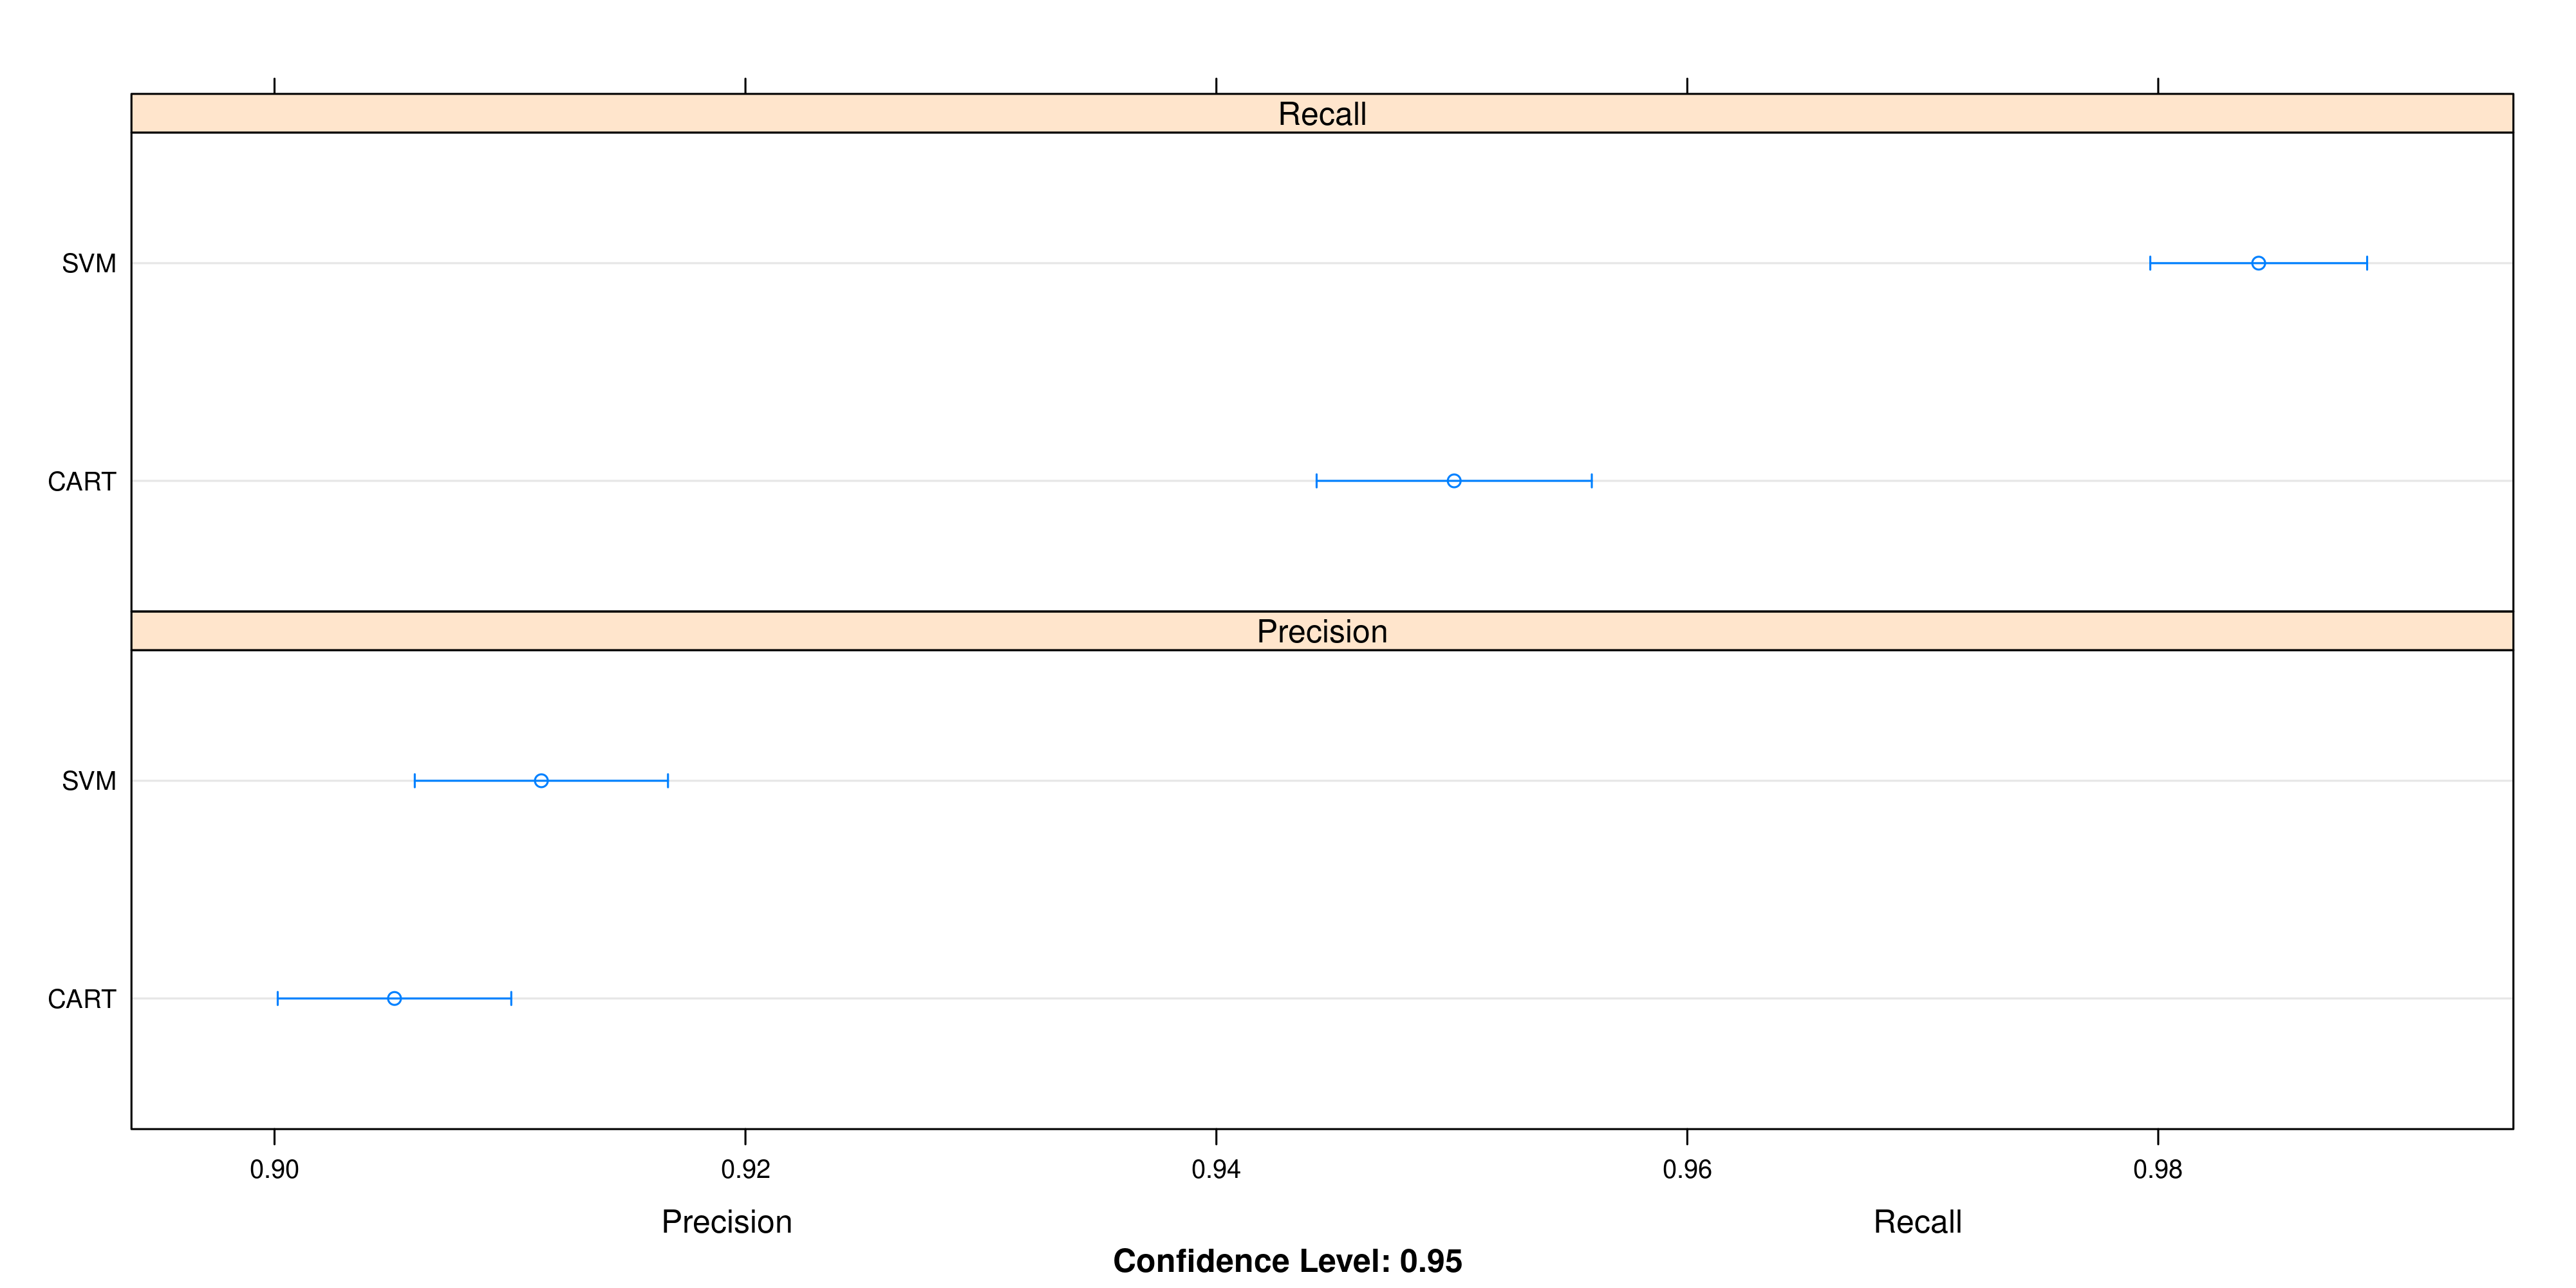
\includegraphics[width=\linewidth]{images/comparison/best/best_dotplot_pr.png}
     \label{fig:c21_modelli_proposti}
    \caption{Intervalli di confidenza dei modelli proposti per Precision e Recall, (svmRadial: svm radiale, rpart2: cart)}
\end{figure}

\noindent
Dagli intervalli di confidenza al 95\% sono visibili leggere differenze in Precision e F1, si può notare una differenza maggiore nella Recall. CART ha un CI molto grande rispetto all'AUC.

\vspace{5mm}
\noindent
Infine osservando i tempi di addestramento vediamo come CART prevede un tempo molto basso di 8.649s, al contrario l'SVM radiale prevede un costo più oneroso di 1827.793s. Dovendo scegliere un modello tra i due proposti l'SVM risulta migliore, nonostante abbia performance simili a CART ed un costo più elevato, poiché CART ha un intervallo di confidenza al 95\% troppo grande rispetto all'AUC.

